\documentclass[12pt,a4paper,norsk]{article}
\usepackage[norsk]{babel}
\usepackage[utf8]{inputenc}
\usepackage{listings}
\usepackage{natbib}
\usepackage{graphicx}
\usepackage{hyperref}

\usepackage{pdfpages} %For å legge til vedlegg som pdf-filer

\usepackage{dirtytalk}
\usepackage{changepage}

\usepackage{nicefrac}

\usepackage{attachfile}

\hypersetup{
    colorlinks,
    citecolor=black,
    filecolor=black,
    linkcolor=black,
    urlcolor=black
}

\title{IT1901 \\ Prosjektrapport}
\author{Gruppe 08\\
    755200, 741068, 757688,\\
    757676, 755591, 757787,\\
    757701, 757734, 757770}

\renewcommand{\contentsname}{Innhold}
\renewcommand\refname{Referanser}

\begin{document}
	\pagenumbering{gobble}
	\maketitle
	\newpage
	\pagenumbering{arabic}
	\tableofcontents
	\newpage
	\section{Introduksjon}

%For referanser skriv [\cite{referansenavn}]
%og om du vil oppgi sidetall \cite[side 1-3]{referansenavn}

%%For å inkludere bilder i rapporten må du legge bildet i img-mappen og inkludere bildet på en slik måte:
%	\begin{figure}[h!]
%  		\includegraphics[width=\linewidth]{img/image00.png}
%  		\caption{Scrum Task-board, with burndown chart}
%  		\label{fig:task-board}
%	\end{figure}
%Så må du huske å referere til figuren i teksten. Eks:
%	Figur \ref{fig:task-board} viser...


%tabeller

%\begin{table}[H] %H forteller latex at tabellen. krever at pakken "float" brukes
%   \centering
%   \begin{tabular}{|p{7cm}|p{3cm}|p{2cm}|}\hline% %formatet || brukes for å merke en celle
%        Sprints & Brukerhistorie & Estimat\\\hline\hline
%%        \csvreader[late after line=\\\hline]%
%        {vedlegg/releaseplan/sheet_v1.csv}{Sprints=\Sprints,  Brukerhistorie-ID=\Brukerhistorie, Estimat=\Estimat}%
%        {\Sprints & \Brukerhistorie & \Estimat}%
%    \end{tabular}
%   \caption{Se oversikt på teknisk stand av koier}
%\end{table}


Dette prosjektet er et gruppeprosjekt gitt i emnet IT1901 - Informatikk prosjektarbeid 1, ved NTNU, høsten 2015. Målet med prosjektet og emnet er å gi deltagerne et innblikk i hvordan det er å jobbe med større gruppeprosjekter og  arbeidsmetoder hvor en tredjepart er med i prosessen. I dette prosjektets tilfelle er tredjeparten en kunde, som skal ta i bruk programmet. Prosjektet skal lære hvordan gruppeprosjekter gjennomføres og gi erfaringer rundt programmeringsverktøy, arbeidsmodeller og den smidige arbeidsmetoden \textit{Scrum}. %Ref?

\subsection{Problemstilling}

Gruppen skal utvikle et administrasjonssystem for NTNUI Koiene. Systemet skal være et tillegg til NTNUI sine eksisterende websider, og gjøre det enklere å drifte koiene. Det skal for eksempel være mulig for en bruker å rapportere vedstatus og ødelagte ting, samt få beskjed om å ta med seg ting til en reservert koie. Medlemmer av Koiestyret skal kunne se disse rapportene og bruke de til å planlegge veddugnader og reparasjoner.

Dette programmet skal gruppen utvikle etter kundens ønsker og behov. Kunden har tildelt en rekke brukerhistorier som skal være oppfylt i det ferdige produktet.

\section{Gruppen og rutiner}
	
\subsection{Rutiner og timeplan}

Det første gruppen måtte løse var timeplanen for prosjektet. Ettersom en studentarbeidsuke er på 40 timer, og vi har 4 emner i semesteret, bestemte vi som gruppe for å møtes og jobbe sammen noe under 10 timer, fordelt på 3 dager i uka.

\begin{itemize}
  \item[] Mandager fra 9:15 - 11:00 
  \item[] Torsdager fra 8:30 - 12:00
  \item[] Fredager fra 10:15 - 14:00
\end{itemize}


%%Litt uklart start på setningen her... og generelt en alt for lang setning.
%Dette fordi det gikk opp med de forskjellige timeplanene og gruppen var innstilt på at korte økter som dette ville holde produktiviteten på de timene oppe og konstruktive. 


\subsection{Gruppen og ansvarsfordeling}
Gruppen bestemte seg tidlig for at alle skulle jobbe med forskjellige arbeidsoppgaver, men ikke låses i fastsatte roller. Dette gjorde vi for å dele kompetansen så mye som mulig og la alle få erfaring i de forskjellige aspektene ved prosjektet. På den måten får man gjort seg mindre avhengig av enkeltpersoner og får aktivisert gruppemedlemmer så mye som mulig.

	\section{Arbeidsprosess}
	\subsection{Scrum i teori}
	\textit{Scrum} er et rammeverk for å utvikle eller videreutvikle produkter, og er veldig populært innen software-utvikling. \textit{Scrum} er en smidig metode, og har som alle smidige metoder fokus på å respondere på endringer og samarbeid med kunden i løpet av prosjektets gang [\cite{agilemanifesto}].
	
	I et utviklingsprosjekt har man gjerne to parter: kunde og utvikler-team. I \textit{Scrum} har man et \textit{Scrum}-Team med en produkteier, en \textit{Scrum}-master og utviklere (se avsnitt \ref{scrumroller} om \textit{Scrum}-roller). Produkteier er kundens representant i \textit{Scrum}-teamet. Produkteier jobber i samarbeid med utvikler-gruppen, ikke bare i planleggingsfasen av prosjektet, men også regelmessig under utvikling.
	[\cite{scrumguides}]
	\subsubsection{Produkt-backloggen}
	Produkteier stiller krav til prosjektet i form av en liste med brukerhistorier. Brukerhistorier er en kort forklaring av hva som skal kunne gjøres med et mål.  Brukerhistorier skrives ofte på formen “Som X skal jeg kunne Y for å Z”, hvor X beskriver brukertypen, Y handlingen brukeren skal kunne utføre og Z målet brukeren har med å utføre handlingen \cite[side 9]{kniberg}. Denne listen med brukerhistorier kalles for produkt-backloggen.
	%Mål?

    Backloggens brukerhistorier får en ID og et kort beskrivende navn. De blir vurdert fra viktigst til minst viktig, på bakgrunn av produkteiers prioriteringer og ønsker, men med eventuelle innspill fra utvikler-teamet.
	\subsubsection{Sprintplanleggingsmøtet}
	Utviklingsfasen deles opp i sykler, og blir i \textit{Scrum} kalt sprinter. I begynnelsen av hver sykel har man i \textit{Scrum} et sprintplanleggingsmøte. Deltakerne på møtet er ikke bare medlemmer av utviklingsteamet med \textit{Scrum}-master, men også produkteier. Formålet med møtet er å forberede og justere produkt-backloggen og planlegge neste sprint.

    \textit{Scrum}-teamet avgjør hvor lang sprinten skal være og finner ut hvilke ressurser man har på denne sprinten. Gruppen avtaler tidspunkt for når på dagen gruppen skal ha det daglige \textit{Scrum}-møtet, når retrospektiv-møtet for sprinten skal være og når demonstrasjonen for produktet skal være \cite[side 16]{kniberg}.
	\subsubsection{Release-plan}
	I noen prosjekter kan det være hensiktsmessig å planlegge lengre frem i tid enn kun for den neste sprinten. Man lager en releaseplan for hele prosjektet. Hensikten med denne er å gjøre det samme som i sprintplanleggingsmøtet, men for alle brukerhistorier. Etter at en sprint er ferdig har man et sprintplanleggingsmøte der man justerer release-planen utifra eventuelle endringer og hvordan sprinten faktisk gikk \cite[side 95 - 101]{kniberg}.
	\subsubsection{Daglig Scrum}
	I \textit{Scrum} har man et daglig møte der hver person svarer på de tre spørsmålene:
	\begin{itemize}
    \item[1.] Hva gjorde jeg sist gang som hjalp gruppen å nå sprintmålet?
    \item[2.] Hva skal jeg gjøre i dag for å hjelpe gruppen å nå sprintmålet?
    \item[3.]   Ser jeg noen eventuelle utfordringer for meg eller gruppen, som kan hindre oss i å nå sprintmålet?
    \end{itemize}
    \textit{Scrum}-møtet skal være kort, med fokus på å få hjelp om man har noen utfordringer.
	\subsubsection{Retrospektiv-møtet}
	Retrospektive møter en en viktig del av \textit{Scrum}. Retrospektiv-møtet er gruppens mulighet til å forbedre prosesser og arbeidsrutiner. Retrospektiver har man på slutten av hver sprint, og både utviklingsgruppen, \textit{Scrum}-master og produkteier deltar. På møtet diskuterer man og svarer på følgende spørsmål:
	\begin{itemize}
    \item[1.] Hva gikk bra i løpet av denne sprinten?
    \item[2.] Hva gikk mindre bra i løpet av denne sprinten?
    \item[3.] Hva kan gruppen gjøre bedre neste sprint?
    \end{itemize}
    Det siste punktet er det som er hovedfokuset i møtet. Det er viktig å komme med konkrete eksempler slik at man er helt sikker på hva det er man kan endre på til neste gang. Retrospektiv skal være den tryggeste måten for gruppen å få frem sin mening, det er derfor viktig at alle i gruppen blir hørt og at ingen skal føle at de ikke kan si sin mening. En måte å få til dette på er at man en etter en får si sin mening om sprinten, uten at noen andre avbryter eller kommer med kommentarer til det som blir sagt. Etter at alle har fått sagt det de vil, så kan man diskutere i gruppen hva som er viktigst å fokusere på å forbedre neste sprint. Da kan man velge ut noen ting som er spesielt viktig å gjøre bedre neste sprint. 

    Disse møtene er viktig fordi det er alltid rom for forbedring i alle grupper. Hvis man ikke har et oppsatt møte der man tar opp hva som har skjedd i sprinten så vil man gjøre akkurat de samme feilene i den neste. Dette gir gruppen muligheten til å forbedre seg utover prosjektet.
    \cite[side 82 - 88]{kniberg}
	\subsubsection{Scrum-roller}\label{scrumroller}
	\textbf {Produkteier}
    \par Produkteier er kundens og eventuelle andre interessenter sin representant. Vedkommende er ansvarlig for å oppdatere  produktbackloggen og for å kommunisere til utviklerne hva brukerhistoriene innebærer.
    [\cite{scrumguides}]
    
    \bigskip \noindent \textbf{\textit{Scrum}-master}
    \par En \textit{Scrum}-master er en tilrettelegger for et produktutviklingsteam som bruker \textit{Scrum} som utviklingsmetodikk, som gir teamet muligheter for selvorganisasjon og håndtering av plutselige endringer under prosjektet. I tillegg til det bruker han/hun \textit{Scrum} for å effektivisere hele arbeidsprosessen og er ansvarlig for at \textit{Scrum} blir brukt som tiltenkt.
 
    \begin{itemize}
    \item[-] Hjelper med å rekke sprintmålene.
    \item[-] Støtter produkteieren med å oppdatere backloggen ved potensielle endringer underveis slik at teamet kan reagere på de.
    \item[-]  Hjelper teamet med å finne en eksplisit definisjon for “done” med vurdering av innspill fra kunden.
    \item[-]  Lærer bort \textit{Scrum}-teknikker til teamet for å sikre at produktet leveres med høy kvalitet.
    \item[-]  Hjelper teamet med å jobbe mer selvstendig.
    \item[-]  Hjelper teamet med å identifisere og unngå eller fjerne             potensielle og faktiske kilder for forstyrring og hindring for både interne og eksterne kilder.
    \end{itemize}
    
    [\cite{scrummaster}]
    [\cite{scrummasterrolle}]
    
    \bigskip \noindent \textbf{Utviklere}
    
    Medlemmene av utvikler-gruppen har ansvar for å gjøre produkt-backloggen om til et fungerende produkt. Utviklere er ikke delt inn i delgrupper. Medlemmer kan ha forskjellige fokusområder, men alle har like mye ansvar for produktets kvalitet. Utviklere ledes ikke av Scrum-master, men får hjelp til å være selvorganiserende.
	
	\subsubsection{Task-board}
	Task-boardet er et verktøy for å gjøre hele arbeidsprosessen mer oversiktlig og interaktiv. Man skal kunne se hvilke brukerhistorier og deloppgaver som må gjøres for inneværende sprint, om noen har begynt på de, om de er ferdige og hvilken prioritet de har. Figur \ref{fig:task-board} viser et eksempel-task-board.
    
    \begin{figure}[h!]
 		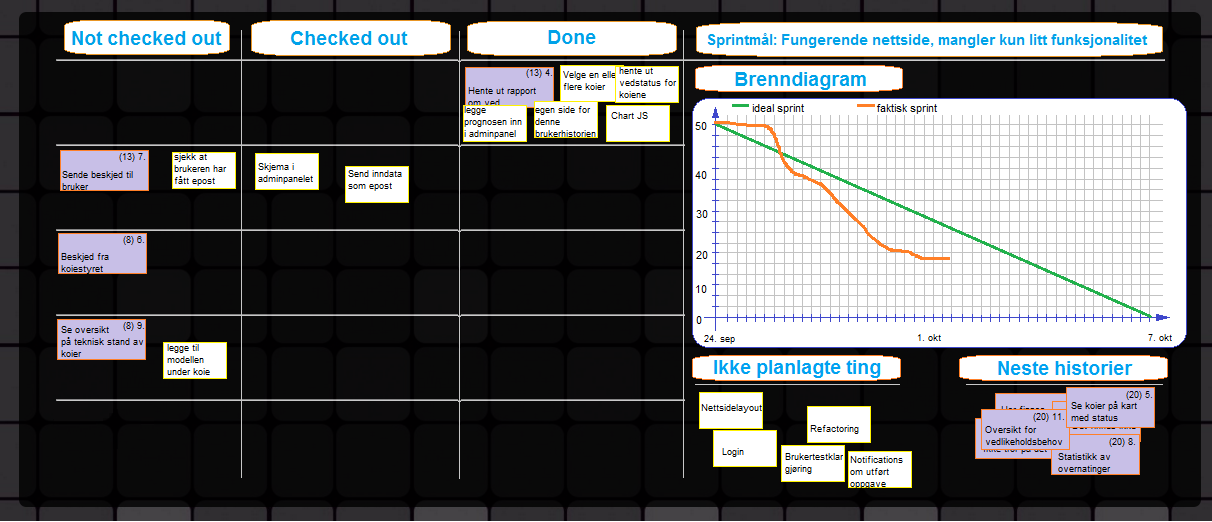
\includegraphics[width=\linewidth]{img/task-board.png}
  		\caption{Eksempel på task-board med brenndiagram}
  		\label{fig:task-board}
	\end{figure}
	
    \textit{Task-boardet} er delt inn i 4 kolonner: \textit{Not checked out}, \textit{Checked Out}, \textit{Done} og \textit{Sprintmål}.
    
    \textit{Not checked out}: Her står brukerhistoriene som ingen har begynt å jobbe med enda. Disse er sortert etter hvor viktig det er å få dem implementert. Der de viktigste står på toppen. En historie er delt opp i flere mindre oppgaver.

    \textit{Checked out}: Her er brukerhistoriene, deloppgavene og “ikke planlagte ting” (se avsnitt om Ikke planlagte ting) som noen har begynt å jobbe med. Det kan også stå hvem som har begynt med den.

    \textit{Done}: Er man ferdig med en brukerhistorie skal den og alle dens deloppgaver ende opp her. Da vet alle som jobber med prosjektet at denne historien oppfyller alle kravene som er nødvendig for at den kan kalles for “ferdig/done”.
	
    \textit{Sprintmål}: Her vises sprintmålet og en seksjonen som er delt inn i tre deler: Brenndiagram, Ikke planlagte ting og de neste historiene i produkt-backloggen.

    Brenndiagram:
    Et todimensjonalt diagram der x-aksen viser datoene fra sprintstarten, sprintslutten og alle datoene i mellom. Y-aksen viser arbeidet som er igjen i storypoints. Så tegner man en graf ut fra hvor man er i sprinten (dato) og hvor mange deloppgaver/brukerhistorier som er blitt fullført denne dagen. Dersom tidsestimatene var riktige ender man opp med en graf som går fra diagrammets venstre topp til høyre bunn i en nesten rett linje.

    Varselsignaler:
	Grafen synker for fort:
    Dersom brukerhistoriene tar mindre tid å implementere enn forventet vil grafen når x-aksen mye fortere enn planlagt. Dette skyldes dårlig estimering og kan løses ved å flytte flere brukerhistorier fra “neste historier”-seksjonen inn i den aktuelle sprinten.

	Grafen synker for sakte:
    Her var estimatene for lave. Brukerhistoriene krever mer tid enn forventet og man henger etter. Måten å løse det er å fjerne en eller flere brukerhistorie fra den nåværende sprinten og flytte dem over til “neste historier”-seksjonen.

    Ikke planlagte ting:
    Her finnes deloppgaver som dukker opp underveis. Disse var ikke planlagt fra starten men må implementeres for at produktet skal fungere.

    Varselsignaler:
	For mange ikke planlagte ting:
    Dårlig planlegging kan lede til en flom av ikke planlagte elementer. Arbeidsmengden øker fortere enn man kan implementere/løse ting som automatisk leder til en for sakte synkende graf.

    Neste historier:
    Her er alle brukerhistoriene som ikke er implementert enda og ikke har fått plass i den nåværende sprinten.
    
    \cite [side 72 -78]{kniberg}


	\subsubsection{Utviklingsverktøy}

\textbf{PyCharm}
\par De fleste på gruppen brukte PyCharm for å jobbe med pythonfilene. PyCharm er et IDE som er mye brukt i programutvikling i Python siden det har mange flere funksjoner enn en vanlig teksteditor som gjør jobben enklere. I tillegg er det mulig å teste koden med en gang i konsollen, samt at det en kan bruke GIT i selve programmet for å holde prosjektet oppdatert.

\bigskip \noindent \textbf{GIT og Stash}
\par For å holde orden på versjoner og endringer i prosjektet brukte vi GIT koblet opp til Stash for å forsikre oss om at ingen endringer og oppdateringer gikk tapt. På Stash hadde vi et repository, dette er litt som en mappe, der hele prosjektet ble laget. I dette repositoriet var det en master-branch, der det nyeste fungerende versjonen av produktet lå lagret, samt flere sidebranches. Man lager en ny sidebranch hver gang man skal jobbe med en ny brukerhistorie eller issue, og når man er ferdig blir denne merget inn i master igjen med de nye endringene. Dette gjør at det er mulig at flere personer jobber med samme kode på forskjellige maskiner samtidig, uten at det blir gjort feil.

I tillegg til at man kan ha flere branches, vil man trenge godkjenning av andre gruppemedlemmer for å merge en ny branch inn i master. Slik kan man være sikrere på at feil i koden blir plukket opp tidlig. Alle endringer som har blitt gjort på prosjektet blir også lagret, så om noe virkelig går galt er det mulig å gå tilbake til en tidligere versjon og å gjøre ting på nytt.


	\subsection{Scrum i praksis}
    Det vil omtrent aldri være mulig å overføre teori direkte til praksis. Kniberg skriver i introen til \textit{Scrum and XP from the trenches} \cite[side 2]{kniberg}:
    
    \bigskip\begin{adjustwidth}{2.5em}{0pt}
    \say {\textit{The strength and pain of Scrum is that you are forced to adapt it to your specific situation}}
    \end{adjustwidth}
    \bigskip Gruppens største utfordring med å tilpasse Scrum var på grunn av forskjellige timeplaner og mangel på et fast og privat rom. I motsetning til en prosjektgruppe i et konsulentfirma ville vi ikke ha muligheten til å møtes hver dag i uka på samme sted.
	
	\subsubsection{Sprintlengde}
	Gruppen bestemte seg for at 2 uker lange sprinter var praktisk fordi vi da kunne møte annenhver uke med veileder for prosjektet og produkteier. I midten av sprinten møtte vi veileder, og i slutten med produkteier. Korte sprinter ville gjøre det mulig for oss å ha retrospektive møter ofte og få tilbakemelding fra produkteier om vi er på rett spor. I slutten av hver sprint var planen å teste funksjonene som hadde blitt implementert i sprinten med produkteier. Dette i form av en brukbarhetstest med scenario-tester.

    Med to uker lange sprinter ville vi oppnå 4 sprinter i løpet av prosjektperioden, med avslutning 4. november. Ettersom innlevering av rapport hadde frist 12. november ville vi ha mulighet etter siste sprint til å jobbe med ferdigstilling av rapporten. 

    For å estimere arbeidskapasitet til hver sprint delte vi opp de timene vi planla å jobbe hver uke i økter. Denne enheten var også den vi ville bruke når vi skulle estimere hvor mange storypoints en brukerhistorie krevde - 1 økt = 1 storypoint. I løpet av en uke ville en person ha 5 økter: mandag: 1, torsdag 2, fredag: 2. Ettersom vi var en gruppe på 9 personer ville vi ha sprinter med 9 (personer) x 5 (økter pr uke) x 2 (uker) = 90 økter pr. sprint. Vi anslo at av 90 teoretiske økter i løpet av en sprint ville ca. 50 økter bli brukt på brukerhistorier. Tallet er lavere på grunn av at noen økter går til møter i gruppen eller med produkteier, mens andre går til rapportskriving, oppsett av utviklermiljø, tid til å sette seg inn i valgte rammeverk eller forbereding til demonstrasjoner og tester. Vi antok at mye av tiden av vår første sprint kom til å gå til planlegging av prosjektet og sette opp utviklermiljø, og anslo at produktive økter kom til å være på ca. 25 økter. Sprint 2,3 og 4 anslo vi til 50 arbeidsøkter, fordi vi antok at vi da kom til å være satt opp med prosjektet, kommet inn i bruk av \textit{Scrum} og klare til å bruke mer tid på utvikling, og mindre tid på administrativt arbeid.

	\subsubsection{Brukerhistorier}
	Produkteier rangerte brukerhistoriene og ga dem lav, høy eller vanlig proritet. Deretter måtte vi rangere disse historiene igjen, for å finne hvilke vi skulle implementere først av de med høyest prioritet. Noen historier så ut til å være avhengige av at andre var ferdige, og måtte nødvendigvis havne i tilsvarende rekkefølge. På grunn av estimater på noen historier måtte vi også gjøre en brukerhistorie med lavere prioritet før en med høyere prioritet, fordi det var den eneste vi fikk plass til i sprinten. 

    Når vi skulle estimere hvor mange arbeidsøkter en brukerhistorie kom til å ta, brukte vi planning poker. Planning poker utføres ved at hver gruppemedlem får en kortstokk med 13 kort, med verdiene 0, \nicefrac{1}{2}, 1, 2, 3, 5, 8, 13, 20, 40, 100, ?, “Pause”. Så velges en brukerhistorie og alle skal individuelt velge ett av kortene som representerer estimert tid for å løse brukerhistorien. Har man bestemt seg for et kort skal den legges på bordet slik at estimatet er skjult. Når alle har et kort liggende foran seg er det på tide å snu dem. Dersom det oppsto store avvik i estimert tid skal man diskutere hvorfor estimatene blir så forskjellige. Deretter skal brukerhistorien estimeres igjen for å se om gruppen blir mer enige om estimatene \cite[side 38-40]{kniberg}.

    Det viste seg å være nyttig. Vi fikk da avdekket at det var forskjellige oppfatninger i gruppen av hva slags tekniske implikasjoner historien innebar. Når en historie ga vidt forskjellige verdier, så kunne de som mente at historien trengte få økter få si hvorfor de mente den ikke trengte så mange og motsatt med de som mente historien trengte mange. Allerede da kom det opp mange gode forslag på hvordan brukerhistorier kan løses på et teknisk nivå. Noen i gruppen visste allerede litt om hva slags muligheter vårt valgte rammeverk ga, og hadde allerede ideer på hvordan spesifikke ting kunne løses. Når vi tok en ny runde planning poker på den samme brukerhistorien fikk vi likere resultat og kunne fastsette antall økter på en brukerhistorie. 

	
	\subsubsection{Vårt Task-board}
	Gruppen bestemte seg for å organisere task-boardet via Trello.com. Trello er et web-verktøy som kan brukes som et digitalt task-board. Alle på gruppen lagde seg en trellobruker, og vi lagde et team som alle på gruppen ble medlem av. Vi inviterte også produkteier til å bli medlem av teamet, så produkteier kunne ha oversikt over hvordan vi lå an, og skrive inn prioriteringer på brukerhistoriene. 

    I Trello kan man lage forskjellige brett, noe vi gjorde for hver sprint. På hvert respektive brett la vi til lister med kort, der hvert kort representerte en brukerhistorie. For hvert brett ble det laget lister for “Not checked out”, “Checked out”, “Andre oppgaver som dukker opp underveis” og “Done”. Etter releaseplanleggingen ble brukerhistoriene lagt inn som kort i “Not checked out” for alle sprintene. 
    
    Når noen skulle begynne på en brukerhistorie, ble det tilsvarende kortet flyttet over til checked out. Trellobrukerne til de som jobbet med brukerhistorien ble knyttet opp mot kortet, så det ble lett å se hvem som jobbet med hva.
    
    Nettlesertilleggene "Scrum for Trello" og "Burndown for Trello" lot oss legge inn estimert tidsbruk og storypoints på et kort, hvor mye tid som faktisk ble brukt på hvert kort, og automatisk generere brenndiagram basert på de to. Se vedlegg Trello-board for forklaring på hvordan vi brukte Trello som task-board.
	\subsubsection{Våre Retrospektiver}
	
\bigskip \noindent \textbf{Retrospektiv Sprint 1}
\par Etter den første sprinten hadde vi satt opp et retrospektivt møte dagen etter vi var ferdig med sprinten. Da satt hele gruppen seg ned og diskuterte hvordan det hadde gått. Alle fikk hver sin tur til å si: “Hva som gikk bra”, “Hva som gikk dårlig” og “Hva vi kan forbedre” (se vedlagt møtereferat: “Retrospektiv Sprint 1”).
 
Hva som gikk bra:
I den første sprinten var gruppen mer effektiv enn vi hadde trodd på forhånd, det resulterte i at vi fikk gjort flere brukerhistorier enn vi hadde trodd. Samarbeidet i gruppen fungerte veldig bra, spesielt at man innad i gruppen hjalp hverandre hvis man ikke fikk til noe. Det gikk også veldig bra å fordele oppgavene opp i gruppen, vi fikk delt oss opp i små grupper som tok hver sine deler og alle tok ansvar for å få gjort sin del. gruppen var også flink til å dele kunnskapen med andre, hvis noen ikke kunne noe så hjalp en annen i gruppen. Dette var veldig lett ved bruk av “mob programming” der vi i små grupper hadde en person som faktisk satt og skrev koden, men flere som kom med ideer og sa hva han skulle skrive. Da kunne de som ikke var helt komfortabel med det nye kodespråket eller programmet være til hjelp uansett, og lære seg noe nytt samtidig. I tillegg så var alle flinke til å lære seg nye teknologier og programmer selv slik at arbeidet gikk fremover. 

Hva som ikke gikk bra:
Helt i starten av prosjektet ble vi enige om at vi skulle gjøre noe sosialt med gruppen hver uke, både for at alle i starten skulle bli bedre kjent med hverandre, og at man skulle få en pause fra de lange øktene med koding og arbeid. Et alternativ som alle var enige i var at vi skulle spise pizza sammen, dette ble ikke gjort iløpet av den første sprinten.  
Et problem har vært at ikke alle i gruppen har kunnet vært med på alle gruppetimene på grunn av sykdom og annet. 
I den første sprinten hadde vi lagt inn god tid til å sette opp utviklingsmiljøet og til å lære seg de forskjellige verktøyene som skulle brukes. Til tross for dette så oppstod det feil etterhvert i sprinten, selv om alt fungerte da vi satt det opp og skulle begynne å arbeide. Dette tok da ekstra tid da vi måtte fikse feilene på datamaskinene før vi kunne fortsette. 
Det var til tider vanskelig å sette allesammen i arbeid den første sprinten, noen hadde problemer og det va ikke alltid nok arbeid til at alle skulle sitte å jobbe hele tiden. Det va også dumt at ikke alle i gruppen fikk prøvd seg på alle de forskjellige oppgavene, slik at man fikk bedre oversikt over hele prosjektet. 
Som sagt tidligere så var vi effektive med oppgavene, det betyr at vi hadde underestimert antallet brukerhistorier vi fikk tid til å gjøre.


Hva vi kan forbedre:
En av de tingene som kom frem at vi kunne bli bedre på var å inkludere alle i flere oppgaver, og passe på at alle til en hver tid hadde noe å gjøre. Vi burde også bytte på hvilke oppgaver vi jobber med i sprinten, slik at alle får kodet og jobbet med rapport.
Vi måtte også bli flinkere på å sette av tid til pauser, da vi også kunne gå ut og spise pizza sammen. 
Når det kom til føring av logg etter møter så var alle enige om at det måtte vi bli bedre på, i tillegg til at vi måtte føre opp hvor mange timer vi hadde brukt på en oppgave, slik at det ble lettere å lage et "brenndiagram".

Vi kom også frem til at vi skulle lage en risikoplan for prosjektet. Der skulle det stå hva vi gjorde når noen fikk problemer med datamaskiner, hvis noen var syk og lignende problemer. Da fikk vi vite kontret hva vi skulle gjøre i de situasjonene. 

Oppsummering:
I denne sprinten var det fokus på å komme igang med prosjektet. Mye av tiden ble brukt til å sette opp datamaskiner, lære mye nytt og til slutt starte på oppgavene. gruppen fant ut hvordan vi skulle jobbe best sammen, både i hele gruppen og i små grupper på de forskjellige oppgavene. Vi har også kommet frem til ting som vi kan gjøre for å forbedre arbeidsprosessen framover. 

\bigskip \noindent \textbf{Retrospektiv Sprint 2}
\par Etter den andre sprinten hadde vi også et retrospektivt møte før vi begynte neste sprint, (se vedlagt møtereferat: “Retrospektiv Sprint 2”). Da gjorde vi det samme som i forrige retrospektivmøte.

Hva som gikk bra:
En av tingene som vi skulle forbedre fra forrige sprint var at alle skulle få mer oversikt over prosjektet. Dette fikk vi til i denne sprinten, vi var flinkere på å inkludere flere i de forskjellige oppgavene, som medførte at alle fikk mer forståelse av koden og bedre oversikt over prosjektet i en helhet. Itillegg til at alle fikk gjøre flere oppgaver så fikk de individuelt oppgaver som matchet deres eget nivå, slik at man fikk utfordringer å overkomme selv.
Iløpet av sprinten så hadde vi fokus på teambuilding i gruppen, vi tok oss en pause fra arbeid og spiste pizza sammen på en fredag, en “tradisjon” som vi fortsatte med utover i prosjektet. Innimellom på møtene prøvde vi også å gjøre noe morsomt sammen, som å se videoer på youtube i pausene. Dette og fokuset på å samle gruppen gjorde at vi føltes med som en helhetlig gruppe som fungerte bedre sammen. 
Generelt er inntrykket at vi jobber bra som en gruppe og ligger godt ann, spesielt siden vi fikk gjort en ekstra brukerhistore da vi gjorde en annen. 
I denne sprinten fikk vi gjort mer enn bare koding i prosjektet, vi fokuserte mer på administrative oppgaver å skriveoppgaver. Vi fikk laget risikoanalyse, utbedret testplanen og har skrevet på rapporten. 

Hva som ikke gikk bra:
I slutten av sprinten fant vi ut at vi hadde litt for stor arbeidsmengde. Det gjorde at vi måtte overføre noen av deloppgavene på ene brukerhistorien til den neste sprinten. 
Et problem som vi merket denne sprinten var at vi fikk mindre ressurser å jobbe med. Det var flere enn tidligere som var borte, noen dro på høstferie og noen var syke iløpet av perioden. Dette var litt av grunnen til at arbeidsmengden ble for stor, itillegg til at medlemmer i gruppen oftere dukket opp seint, slik at det tok lengre tid å komme igang med møtene. 

Hva vi kan forbedre:
Siden mange var borte denne sprinten så var en ting gruppen kunne bli bedre på å finne seg arbeidsoppgaver å gjøre hjemme, og å faktisk prøve å gjøre de.
Itillegg så skal vi ha en person som følger opp de som er borte/seine og ha 1-1 samtaler med dem for å finne bedre ut hvorfor de er seine og hvordan det kan unngås. 

Oppsummering:
I denne sprinten forbedret gruppen seg på noen av de punktene som vi skulle jobbe med fra forrige sprint, som at alle skulle få delta på mer på forskjellige oppgaver. Til forskjell fra den forrige sprinten der gruppen overestimerte tiden på brukerhistoriene så ble det noen oppgaver igjen etter denne sprinten på grunn av mye fravær. 

\bigskip \noindent \textbf{Retrospektiv Sprint 3}
\par Etter den tredje sprinten hadde vi også et retrospektivt møte før vi begynte neste sprint, (se vedlagt møtereferat: “Retrospektiv Sprint 3”). Da gjorde vi det samme som i de forrige retrospektivmøtene. 

Hva som gikk bra:
En av tingene som har gått bra denne sprinten er at flere i gruppen har tatt mer ansvar for sitt eget arbeid, har vært flinkere til å finne seg oppgaver å gjøre og å være mer engasjert i prosjektet. Spesielt har det gått bra å jobbe hjemmefra når noen i gruppen har vært syk, kommunikasjonen mellom de som har vært borte og gruppen har vært så bra at dette har gått smertefritt. Dette viser god forbedring fra forrige sprint da vi ville bli bedre på akkurat dette, mye fordi vi har hatt en person som følger opp de som er borte. 
Gjennom sprinten så har gruppen vært effektiv med de arbeidsoppgavene vi har hatt, det vises ved at de oppgavene som var igjen fra forrige sprint, de fra denne sprinten og deler av neste sprint har blitt gjort. Dette er mye fordi alle har vært flink til å finne enkle løsninger på de oppgavene som har blitt gjort. 
Itillegg til brukerhistorier og design har gruppen også gjort noe morsomt på nettsiden med noen gjemte funksjoner, også kalt “easter eggs”.  

Hva som ikke gikk bra:
En av de tingene som har gått dårlig i denne spriten er at gruppen har vært dårlig på å estimere tid på brukerhistoriene, vi trodde det kom til å gå lengre tid på dem. Dette var fordi ingen hadde god nok kjennskap til de ulike verktøyene som skulle brukes til å gjøre et mer riktig estimat, f.eks. for å lage kart på en nettside.
I sprinten så ble det for dårlig fokus på å føre opp timer som ble brukt på de forskjellige oppgavene og å skrive logg for hva som skjedde på hvert møte. 
Et problem var at flere i gruppen ble syk og var borte flere ganger enn tidligere, men en i gruppen tar alltid kontakt hvis noen er borte og ikke gir beskjed, slik kan de få oppgaver å gjøre hjemme. 
Mot slutten av sprinten så var mye av arbeidet ferdig, da var det generelle inntrykket i gruppen at alt var ferdig. Det gjorde at man slappet litt mer av og ikke jobbet like hardt som var ønskelig, iallefall siden det viste seg at det var problemer med noen av funksjonene som vi måtte fikse i neste sprint. 
Når det kom til rapporten så mente flere i gruppen at det var vanskelig å vite hvordan man skulle skrive en bra rapport, det førte til at deler av rapportskrivingen gikk sakte da man satt seg fast.

Hva vi kan forbedre:
Vi har sett tidligere at en logg for hvert møte kan være bra for dem som er borte en dag så de får oversikt over hva som har blitt gjort mens de var borte. Selv om denne kommunikasjon har gått bra denne sprinten så er det fortsatt ønskelig å ha en logg til senere, så dette er et punkt gruppen må bli bedre på til neste sprint. 
Et annet punkt gruppen kan bli bedre på er å holde de møtene vi har fokusert på de oppgavene som må gjøres, til tider hender det at fokuset drifter over på ting som ikke er så viktig. Siden det fortsatt er mye fravær og forseintkomminger så ville det vært bra for gruppen at alle blir flinkere til å komme til tide, kanskje ved å sette på 2 alamer på morgenen.   
Noe som er veldig viktig er at man tester funksjoner bedre før man skriver at de er ferdig, da slipper gruppen å tro at alt er ferdig når det fortsatt er feil i funksjoner. 

Oppsummering:
I denne sprinten så har gruppen jobbet både bra og dårlig. Oppgavene ble gjort “ferdig” tidlig, men på grunn av dårlig testing så visste vi ikke om feilene før mot slutten av sprinten, da ble noen oppgaver overført til neste sprint der det ikke var så mye kodejobb å gjøre. Da gruppen trodde alt var ferdig tidlig ble det stort fokus på skriving av rapporten, dette var positivt da mye av arbeidet på rapporten ble gjort.

\bigskip \noindent \textbf{Retrospektiv Sprint 4}
\par Etter den tredje sprinten hadde vi også et retrospektivt møte før vi begynte neste sprint, (se vedlagt møtereferat: “Retrospektiv Sprint 4”). Da gjorde vi det samme som i de forrige retrospektivmøtene. 

Hva som gikk bra:
I denne sprinten ble vi helt ferdig med produktet, selv om det ikke var mange oppgaver igjen til denne sprinten så er gruppen godt fornøyd med å være ferdig. Dette har vi gjort ved å ha god arbeidsånd mot slutten av prosjektet, det har vært godt oppmøte og mye har blitt gjort. 
Gruppen er også fornøyd med hvor mye som er ferdig på rapporten, og det merkes at det har blitt gjort arbeid på den i tidligere sprinter også. 

Hva som ikke gikk bra:
Noe som gruppen ikke var forberedt på var at det skulle skrives dokumentasjon på all koden, dette var ikke en del av den planen vi la opp mot slutten av prosjektet. 
Selv om vi har jobbet godt og fått gjort mye så har det til tider vært litt dårlig fokus og tull på møtene, det viser bare at det er alltid rom for forbedring. En grunn til dette er at mot slutten av prosjektet begynner folk å bli litt lei og slitne, spesielt når man sitter og skriver rapport i lengre perioder. Gruppen merket til tider at 4 timer i strekk var litt for lange arbeidsmøter, derfor ble de kuttet ned til 2 timer hver gang.
Et problem med å skrive rapport er at vi har skrevet over maksgrensen for ord, som kan føre til at det er noe urelevant og duplisert arbeid. 

Hva vi kan forbedre:
En ting gruppen kunne forbedret var å involvere flere personer i rapportskriving tidligere, slik at det ikke ble like mye å gjøre mot slutten. 
Gruppen skulle også klart å holde bedre fokus på møtene, for å være enda mer effektive. 
En annen ting vi kunne gjort bedre var å endre arbeidsmetoden i denne sprinten, der det for det meste bare var rapportskriving. Fordi måten man jobber best med kode og rapport er ikke nødvendigvis det samme, f.eks. lengde på arbeidsøkter, og man kan gjøre mer hjemme og møtes færre ganger. 

Oppsummering:  
I denne sprinten har gruppen fått gjort mye, både gjort ferdig produktet og skrevet rapport. Vi har funnet noen punkter som vi kunne har gjort annerledes når det kommer til arbeidsmetode og gruppesamarbeid. 

	\subsubsection{Sprintgjennomgang}
\bigskip \noindent \textbf{Sprint 1}
\par I starten av sprint 1 hadde gruppen et sprintplanleggingsmøte, der diskuterte vi hva vi skulle gjøre i sprinten og hvilke brukerhistorier vi skulle få gjort. De brukerhistoriene som ble prioritert i første sprint var de som var satt opp i releaseplanen med høy prioritet fra kunden (se vedlegg: releaseplan v1). Gruppen laget en ny brukerhistorie som man trodde ville ta lang tid å gjennomføre og som ble satt til sprint 4, nemlig administrasjon av koiene på nettsiden. 

Halvparten av arbeidsøktene i sprint 1 var satt opp til å sette opp datamaskiner, da skulle Stash settes opp til alle i gruppen, alle skulle få installert PyCharm og lastet ned Django. Itillegg til dette ble nettsiden som skulle videreutvikles senere laget, og administrasjonsdelen til denne siden ble satt opp. Dette tok ikke så lang tid som det var estimert, det gjorde at det ble mer tid til å kode brukerhistoriene som var satt opp. 

I starten delte gruppen seg opp i to små grupper som tok for seg brukerhistoriene om å rapportere inn ved og ødelagte ting på koiene. Det var fordi disse to var ganske lik, så derfor kunne de to gruppene lære seg det samme, og fortsatt kunne hjelpe hverandre med det som var vanskelig i oppgavene. Dette var det første mange i gruppen gjorde i Django og det var derfor bra å ha noen å spørre om hjelp. Disse brukerhistoriene gikk mye på å lage et skjema der brukere kunne sende inn informasjon, da dette var de første oppgavene som ble gjort tok de litt noe lengre tid enn estimert. Dette jevnet seg ut etterhvert i sprinten, da flere ble komfortabel med Django gikk arbeidet mye fortere. 

Den siste brukerhistorien om at koiestyret skulle kunne ta ut rapporter av ødelagte tok veldig mye mindre tid enn estimert, fordi det var mye enklere da man kom igang med det enn gruppen hadde trodd på forhånd. Dette gjorde at vi hadde tid til overs i sprinten, vi valgte da å overføre brukerhistorien om å rapportene inn tekniske utbedringer på en koie fra sprint 2 til 1.  Vi valgte den fordi den hadde lavest tidsestimat slik at vi var sikker på at vi ble ferdig med den i sprint 1, selv om det var den med lavest prioritet fra kunden. Dette ble også klarert i møte med kunden. 

Brenndiagrammet viser hvordan progresjonen for oppgavene var i denne sprinten (se vedlegg).

\bigskip \noindent \textbf{Sprint 2}
\par I starten av sprint 2 hadde gruppen også et sprintplanleggingsmøte. Vi gikk ut fra releaseplanen for hva som skulle gjøres, men siden en brukerhistorie ble flyttet til sprint 1 ble en hentet fra sprint 3 til sprint 2 også (se vedlegg: releaseplan v2). Da valgte gruppen den brukerhistorien som hadde mest lik estimert tid som den som egentlig var i sprint 2. Brukerhistorien som gruppen laget i forrige sprint om administrasjon av koier ble fjernet, dette var fordi at denne fuksjonen ble implementert nesten av seg selv da andre oppgaver ble gjort, vi valgte da å fjerne den siden det ikke faktisk ble gjort noe arbeid spesifikt på den. Gruppen valgte også i sprint 2 å lage enda en brukerhistorie, den handlet om å starte å designe nettsiden med forside og navigering rundt på siden. Dette gjenspeiler målet for sprinten, som var: Ha en fungerende nettside som kun mangler litt funksjonalitet.

I denne sprinten handlet brukerhistoriene om direkte kontakt mellom koiestyret og brukere, og det å ta ut rapporter for ved og teknisk stand. Her som før ble oppgavene fordelt på mindre grupper. Funksjonene for å ta ut vedrapporter og teknisk stand gikk veldig bra, fordi det lignet på det som ble gjort i forrige sprint.

Den brukerhistorien som var viktigst i sprinten var å kunne ta ut ved rapporter og prognoser for en eller flere koier. Den var litt vanskeligere, dette var fordi man selv måtte definere hvor mye ved som gikk for hver dag koien ble brukt og så lage en graf ut av dette og en prognose for når det blir tomt. 

I denne sprinten ville gruppen bli ferdig med brukerhistoriene som handlet om kommunikasjon mellom koiestyret og brukeren, derfor ble et epostsystem for å melde fra om ting som måtte tas med til og fra koier implementert. 

Arbeidet med nettsiden kom også ganske langt, det ble laget forside og en navigasjonsmeny der de fuksjonene som ble gjort i sprint 1 og 2 ble lagt til. Dette gjorde at nettsiden allerede hadde mye funksjonalitet, blant annet å kunne melde inn ved, ødelagte ting å tekniske utbedringer fra brukeren, og at koiestyret kunne hente ut rapporter for dette. 

I slutten av sprinten ble det funnet noen bugs i vedprognosefunksjonen som det ikke ble tid til å gjøre iløpet av sprinten, disse ble derfor overført til den neste sprinten.

Brenndiagrammet viser hvordan progresjonen for oppgavene var i denne sprinten (se vedlegg).

\bigskip \noindent \textbf{Sprint 3}
\par I starten av sprint 3 hadde gruppen også et sprintplanleggingsmøte. Vi gikk ut fra releaseplanen for hva som skulle gjøres (se vedlegg: releaseplan v3). I denne sprinten var det kun 2 brukerhistorier, men tidsestimatet på dem var det høyeste som var gitt noen brukerhistorier. Itillegg til disse så hadde gruppen oppgaver fra forrige sprint som måtte gjøres ferdig, og mye arbeid med å få nettsiden til å se ferdig ut. Det var også på tide å vise frem en demonstrasjon av produktet til nå. 

For brukerhistorien om å få oversikt over vedlikedholdbehov utfra forventet levealdre på konstruksjonen av koien var det noe usikkerhet på hvordan den skulle gjøres. Om man måtte gå gjennom alle koiene å finne ut når de ble bygget, oppusset og når de trengte å gjøres noe med. Da dette ville kreve mye arbeid, å det ikke var sikkert at man ville finne ut av det i det hele tatt. Etter å ha snakket med kunden kom man frem til en bedre løsning der man istedet legger inn når noe er reparert/satt inn nytt og hvor lenge disse vil vare, så kan man se på nettsiden når de må gjøres noe med igjen. 

For brukerhistorien om å lage et kart over koiene med status over utstyr og ved så var oppgaven forståelig, men selve utføringen med å lage kartet tok litt tid siden det var noe helt nytt å sette seg in.. Vi løste oppgaven ved å lage kartet med riktige posisjoner på koiene, og at man kan trykke på hver koie og få opp link til vedstatus og utstyr. Her fikk vi en bug der man ikke kom til riktig koie på linkene, som ikke ble løst før i sprint 4.   

Begge disse brukerhistoriene tok mye mindre tid enn estimert, derfor bestemte gruppen seg for å hente den siste brukerhistorien fra sprint 4 og gjøre den. På den skulle koiestyret få oversikt over overnattinger på koier i et gikk område. Får å gjøre dette laget vi et script som hentet informasjonen om overnattinger fra NTNUI sine nettsider, deretter laget vi soner på kartet med de forskjellige koiene og la sammen overnattinger for hver sone som vises under kartet. 

Det ble også jobbet med nettsiden denne sprinten, spesielt med å endre administrasjonsiden slik at den ble lettere å forstå, og å gjøre nettiden mer brukervennlig.  

Brenndiagrammet viser hvordan progresjonen for oppgavene var i denne sprinten (se vedlegg).

\bigskip \noindent \textbf{Sprint 4}
\par I starten av sprint 3 hadde gruppen også et sprintplanleggingsmøte. Vi gikk ut fra releaseplanen for hva som skulle gjøres. I denne sprinten var det ingen brukerhistorier igjen, den som var planlagt å gjøre her ble overført til forrige sprint istedet (se releaseplan v3). Dette gjorde at de oppgavene som skulle gjøres gikk mer på finpussing av nettsiden og testing av systemet generelt, som reflekteres i målet for sprinten: Få et fullstendig produkt, hvor produktets funksjoner oppleves intuitivt for brukeren.

Nettsiden ble endret på flere måter, nå som gruppen hadde god tid ble kartene som allerede var implementert i tidligere brukerhistorier endret. Dette var fordi vi ville ha en finere løsning, og fordi det var en bug med linkene fra kartet til status på koiene som også måtte fikses. Det ble også gjort flere endringer i designet på siden, som å endre navn på linker til å være lettere å forstå hvor de gikk. Etter å ha snakket med kunden ble også posisjonen av kartet og informasjonen om overnattinger flyttet på for å få bedre oversikt. 

Bortsett fra dette gikk tiden til å skrive rapport, testing, skriving av dokumentasjon og utføring av akseptansetest med kunden. 

Brenndiagrammet viser hvordan progresjonen for oppgavene var i denne sprinten (se vedlegg).

	
	\section{Risikoanalyse}
	Tidlig i prosjektet bestemte gruppen seg for at det var en god ide å skrive en risikoanalyse for hvilke faktorer som kunne hindre fremgangen i gruppen. Alle risikofaktorene er tilgjengelig i tabellform under vedlegg, (“risikoanalyse”). En viktig fordel for gruppen var at den bestod av mange gruppemedlemmer, så dermed kunne gruppen ta ansvar for å sette seg inn i og utføre arbeidsoppgaver ved fravær. Dette utspilte seg positivt, da flere fikk satt seg inn i andre deler av prosjektet.
	
	\section{Produkt}
	Før vi bestemte oss for hvilken løsning vi skulle velge for produktet, gikk vi over brukerhistoriene vi hadde fått for å vurdere hva som ville passe best for kunden. Etter å ha vurdert både desktop-program i JavaFX og en mobilapp, valgte vi å gå for en nettside. Hovedgrunnen er at en nettside er lett tilgjengelig på både mobil og datamaskin og krever ingen installering for brukeren sin del. Gruppen valgte å bruke webrammeverket Django som utviklingsplattform. Se vedlegg "Django" for beskrivelse av hvordan komponentene i Django fungerer.
	
	I vår implementasjon rapporterer koiebrukere status på koiene ved å fylle ut forskjellige skjemaer og sende de inn. Dette innebærer vedstatus, vedlikeholdsbehov, forslag til tekniske utbedringer og reparasjoner for hver eneste koie. Brukere må fylle inn eposten sin for å sende en rapport.
	
	Medlemmer av Koiestyret har mulighet til å logge seg inn på en adminside som har oversikt alle rapportene. Denne kan brukes til å blant annet planlegge veddugnader basert på vedprognoser eller reparasjoner. Kommunikasjon fra administrasjonen til koiebrukerne foregår via epost. Se vedlegg "Brukermanual" for en detaljert beskrivelse på hvordan produktet fungerer. 
	
	Løsningen vår kan testes på IP-adressen http://178.62.64.191/. Se vedlegg "Teknisk brukermanual" for hvordan nettsiden kan settes opp på kundens egen server.
	
	\section{Testing}
%           produktet, systemet, brukerhistoriene
Når gruppen skulle teste produktet ble det valgt å ikke bruke unit tester i Python, men heller å fokusere på å teste brukerhistoriene selv. Dette ble gjort i form av brukbarhetstester for kunden, og ved å skrive et testdesign dokument der hver brukerhistorie ble testet. Testdesignet består av hvordan testene ble gjennomført, og hvilke tilbakemeldinger en forventet ved gyldig/ugyldig data som føres inn.
%data som føres inn, hjelp meg på den
I tillegg har debug modusen til Django blitt benyttet gjennom hele prosjektet, fordi koden måtte fungere for å få vist nettsiden. Debug modusen blir benyttet ved å sette debug = True i settings.py filen, og tilbyr en detaljert visning av feilmeldingene som kan oppstå.

I Knibergs bok under kapittelet om testing\cite[side 128-131]{kniberg}, blir det fortalt om viktigheten med testere i et \textit{Scrum} team. Det sies også at et \textit{Scrum} team, sett bort fra \textit{Scrum}-masteren, skal være rolleløs og kryssfunksjonell. Hvor hele teamet bidrar med testingen, og samtidig er det en som tar mer ansvar når det gjelder testing og kjører mere komplekse tester. Dette medfører at hele teamet blir involvert i testingen, som er positivt fordi hele teamet er ansvarlig for produktkvaliteten.

 \subsection{Brukbarhetstester}
Etter hver sprint skulle det som ble fullført i den avsluttende sprinten testes for kunden i form av brukbarhetstester. Brukbarhetstesten ble gjennomført av kunden og bestod av å løse scenario oppgaver på nettsiden relatert til de brukerhistoriene som ble fullført den sprinten. Hele gruppen var tilstede under testingen, men det var to personer som hadde hovedansvaret for testen, disse dannet hovedrollene testleder og observatør. Testlederen hadde ansvaret for å hjelpe kunden gjennom oppgavene og at testen ble gjennomført. Observatørens oppgave var å observere hvordan kunden brukte produktet, om det var brukervennlig og hva som bør endres på.

Ved å teste målene gruppen oppnådde for kunden, fikk gruppen sett hvordan produktet ble brukt av noen som ikke har jobbet med nettsiden. Dette hjalp til å se om produktet var brukervennlig eller hvilke deler som var forvirrende for kunden. Flere av navnene under administrasjonssiden måtte endres, da disse var misvisende og forvirrende. Det samme gjaldt for linkene på hovedsiden, disse ble senere lagt til i en undermeny kalt 'Rapporter', med endret navn på linkene slik at de tilhørte der. I tillegg under administrasjonmenyen på hovedsiden, hadde vi en link for både kart og statistikk. Kartet viste oversikt over koiene, og statistikk siden viste statistikk, status og sonene til koiene. Disse ble senere slått sammen, og opprettet linken 'Kart og statistikk'.

\newpage
\phantomsection
\section{Referanser}
%\addcontentsline{toc}{section}{Referanser}
\bibliographystyle{agsm}
\bibliography{referanser}
\section{Vedlegg}

%To be clear, you need to specify the pages you wish to include, i.e. \includepdf[pages={1,3,5}]{myfile.pdf} would include pages 1, 3, and 5 of the file. To include the entire file, you specify pages={-}, where {-} is a range without the endpoints specified which default to the first and last pages, respectively.

\addcontentsline{toc}{subsection}{Testplan}
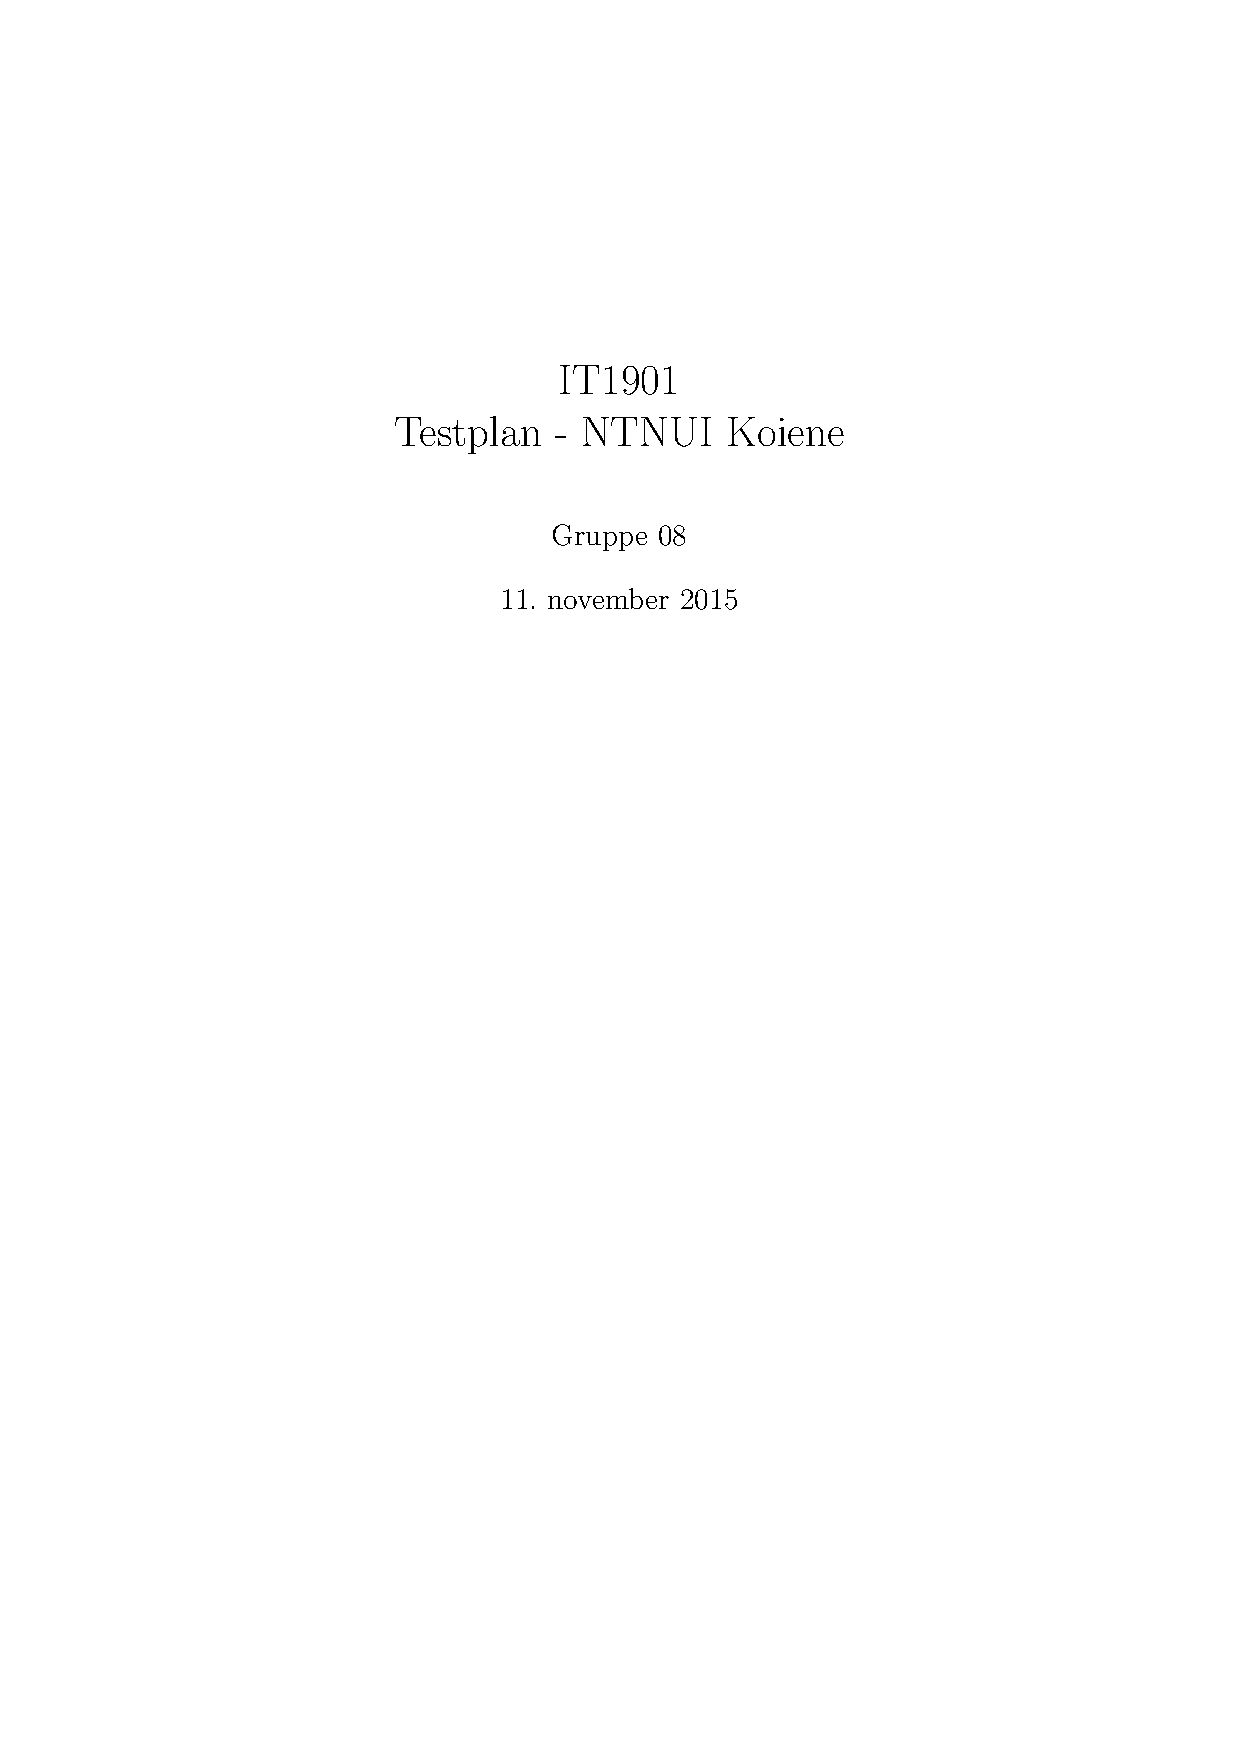
\includepdf[pages={-}]{vedlegg/testplan}

\addcontentsline{toc}{subsection}{Brukbarhetstest}
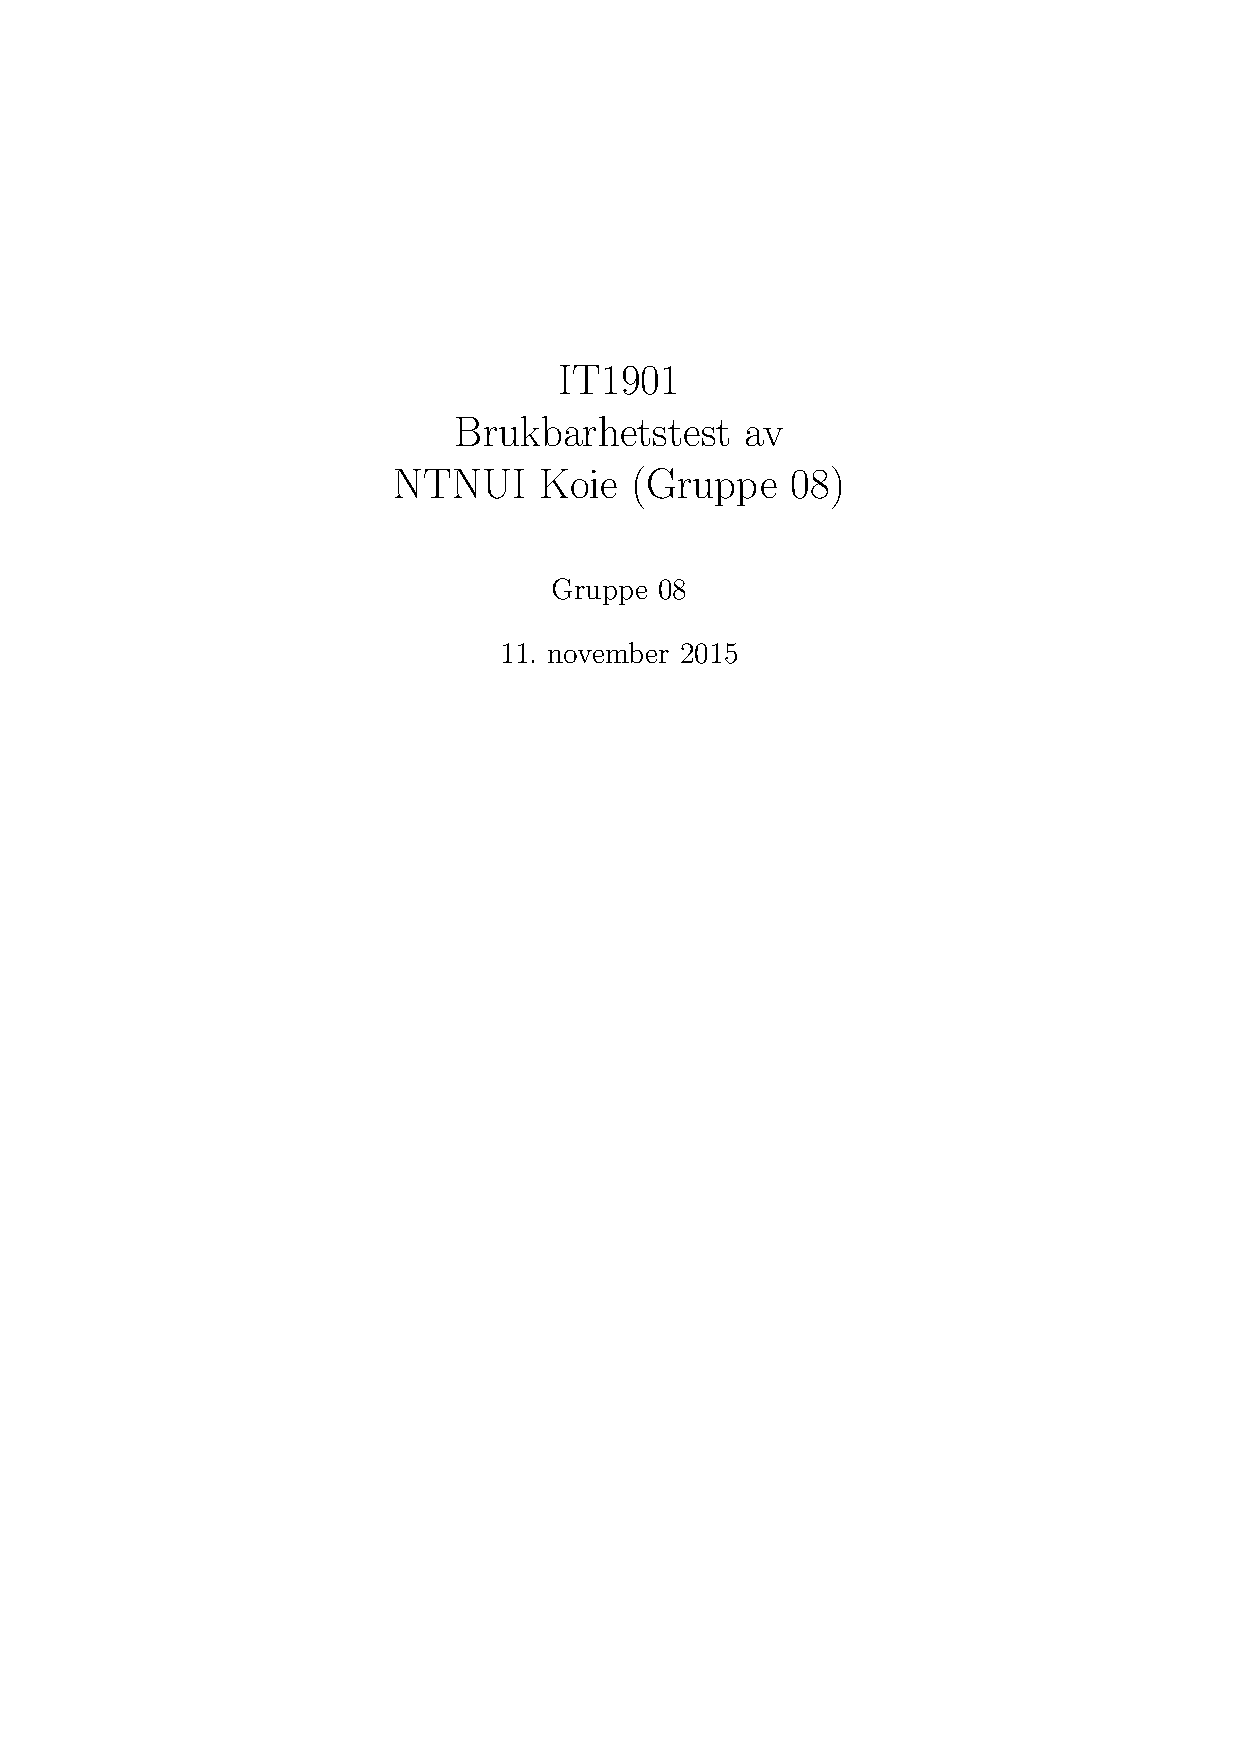
\includepdf[pages={-}]{vedlegg/brukbarhetstest}

\addcontentsline{toc}{subsection}{Brukermanual}

\includepdf[papages=1,gecommand={\subsection{Brukermanual}}]{vedlegg/brukermanual}

\includepdf[pages={2-}]{vedlegg/brukermanual/brukermanual}

%\addcontentsline{toc}{subsection}{Teknisk Brukermanual}
%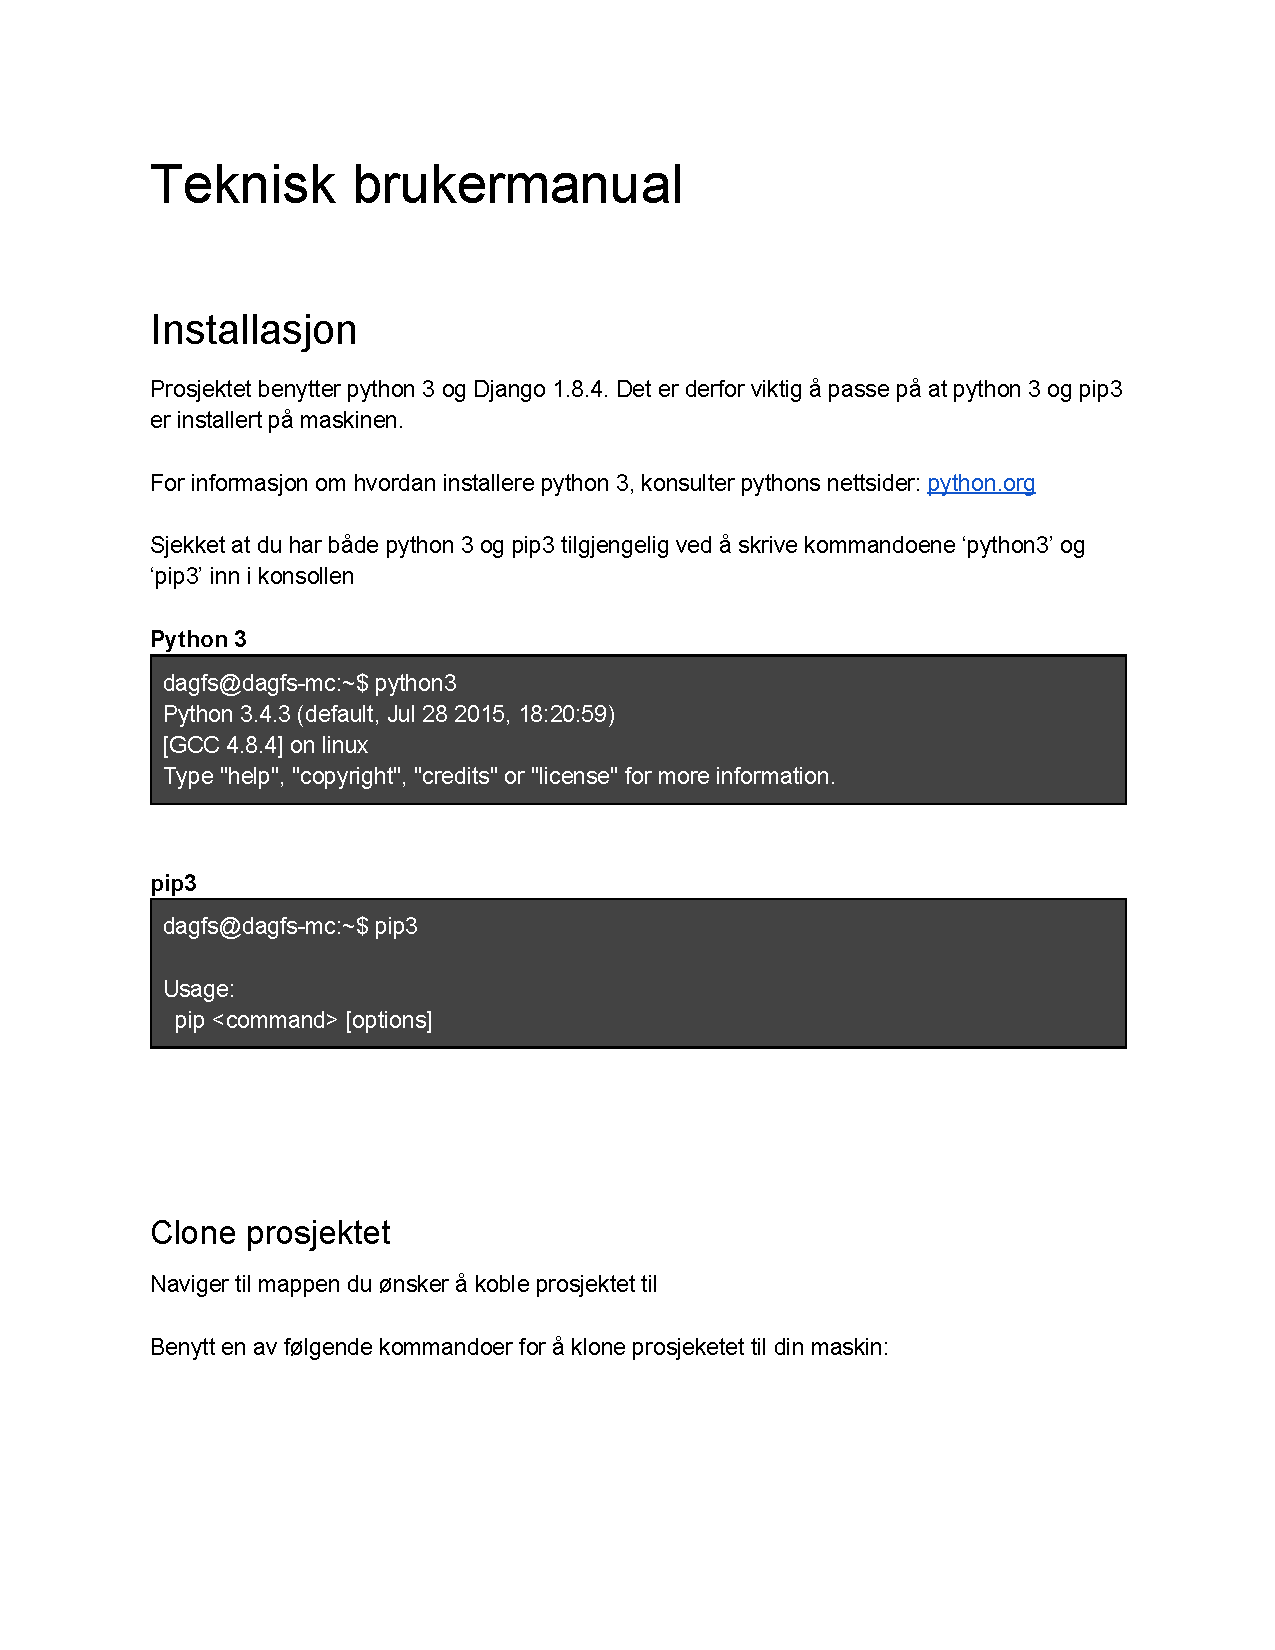
\includepdf[pages= 1, pagecommand={\subsection{Teknisk Brukermanual}}]{vedlegg/tekniskbrukermanual/tekniskbrukermanual}
%\includepdf[pages={2-}]{vedlegg/tekniskbrukermanual/tekniskbrukermanual}

%\addcontentsline{toc}{subsection}{Risikoanalyse}
% ??

%%RETROSPEKTIV
%\addcontentsline{toc}{subsection}{Retrospektiv}

%\addcontentsline{toc}{subsubsection}{Sprint 1}
%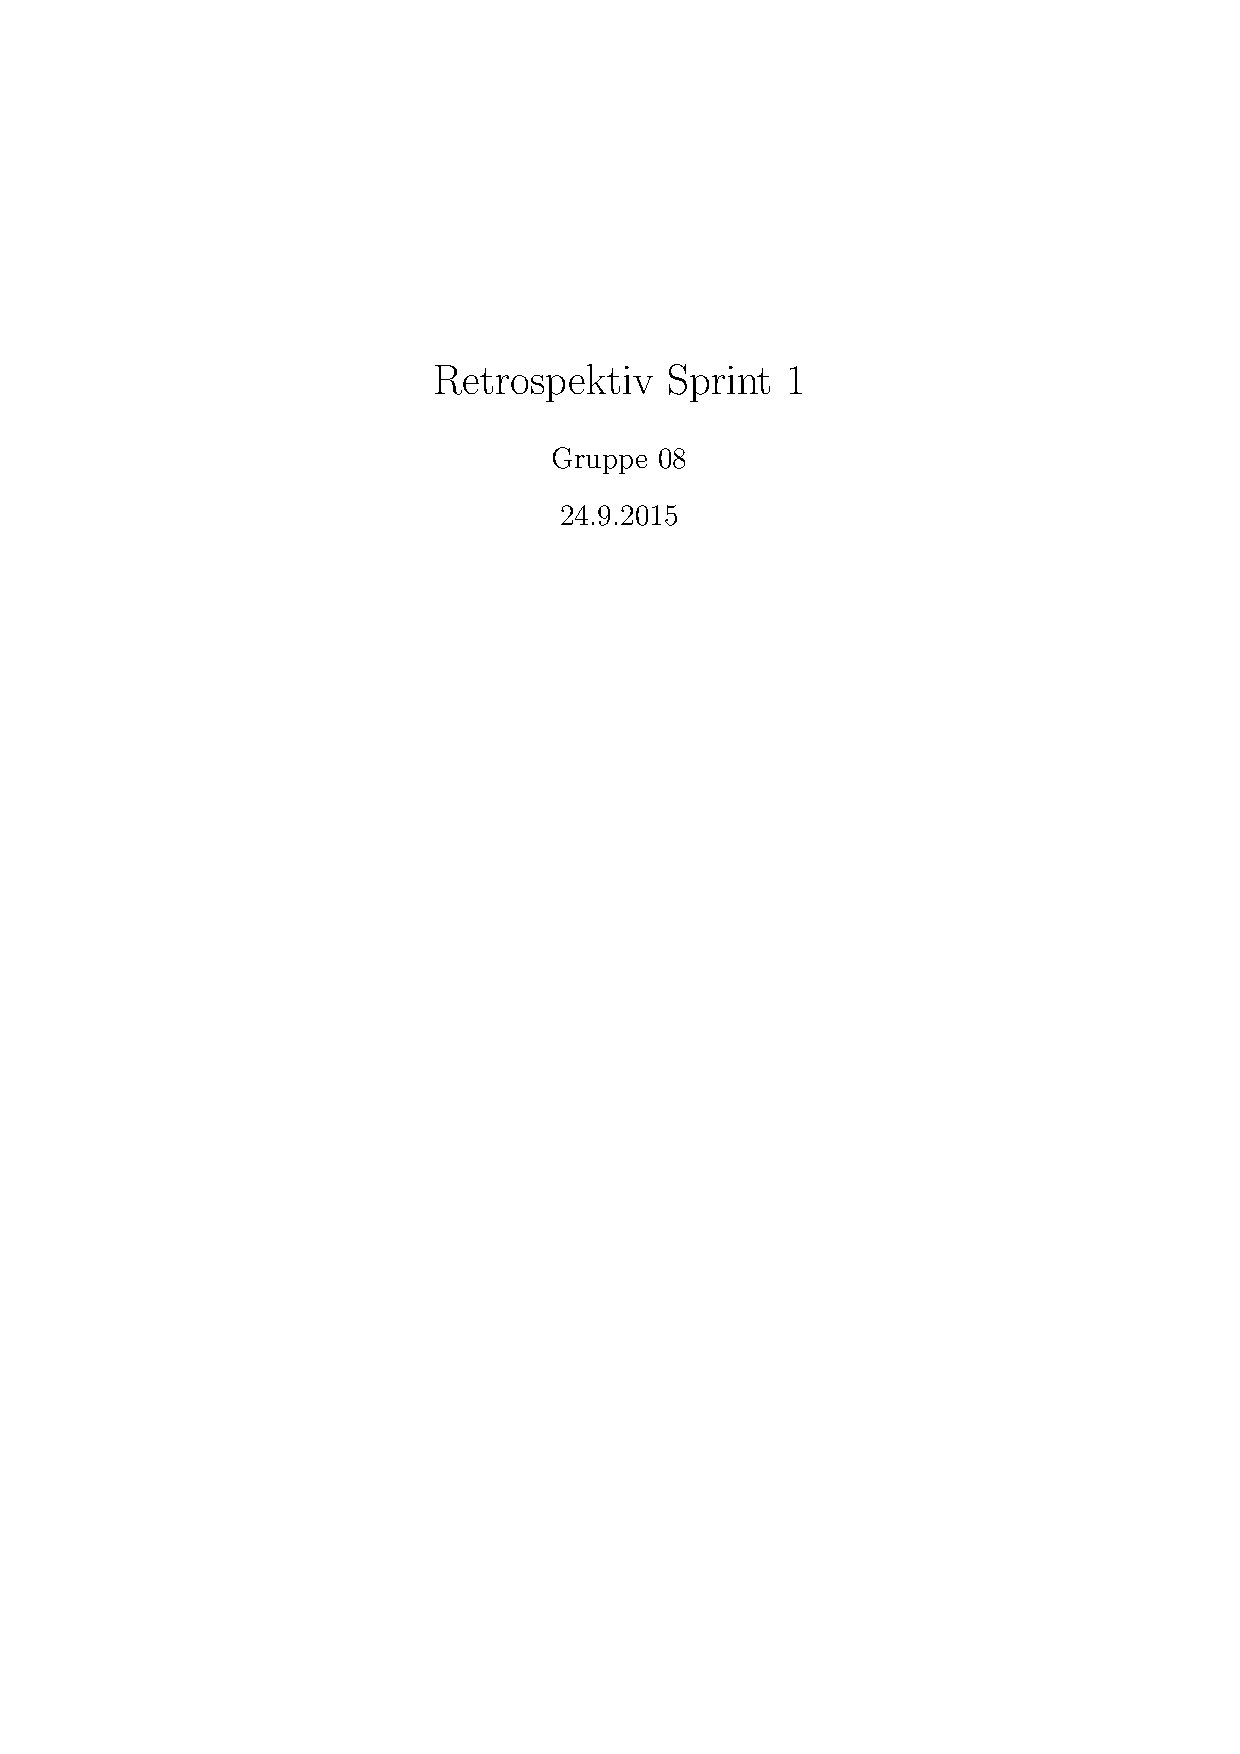
\includepdf[pages={-}]{vedlegg/Retrospektiv/sprint1}

%\addcontentsline{toc}{subsubsection}{Sprint 2}
%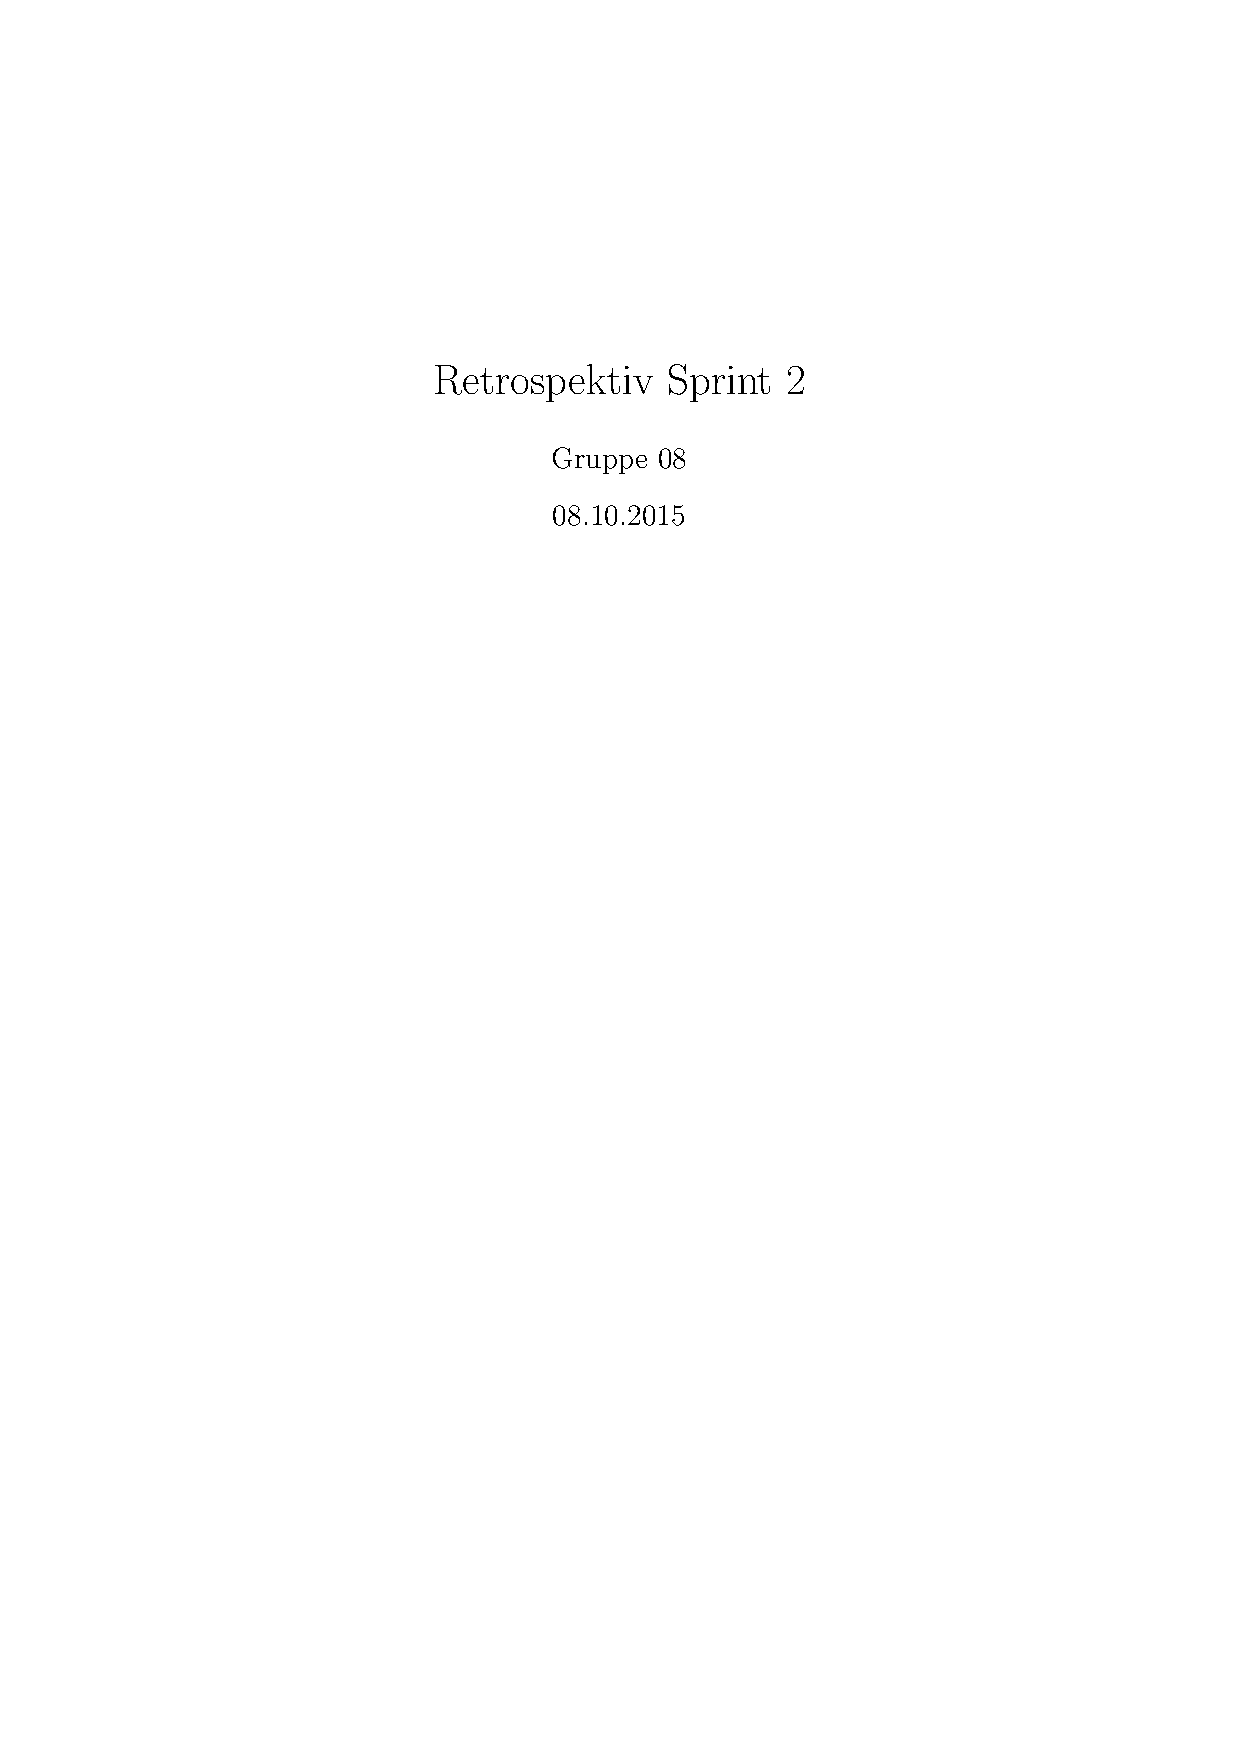
\includepdf[pages={-}]{vedlegg/Retrospektiv/sprint2}

%\addcontentsline{toc}{subsubsection}{Sprint 3}
%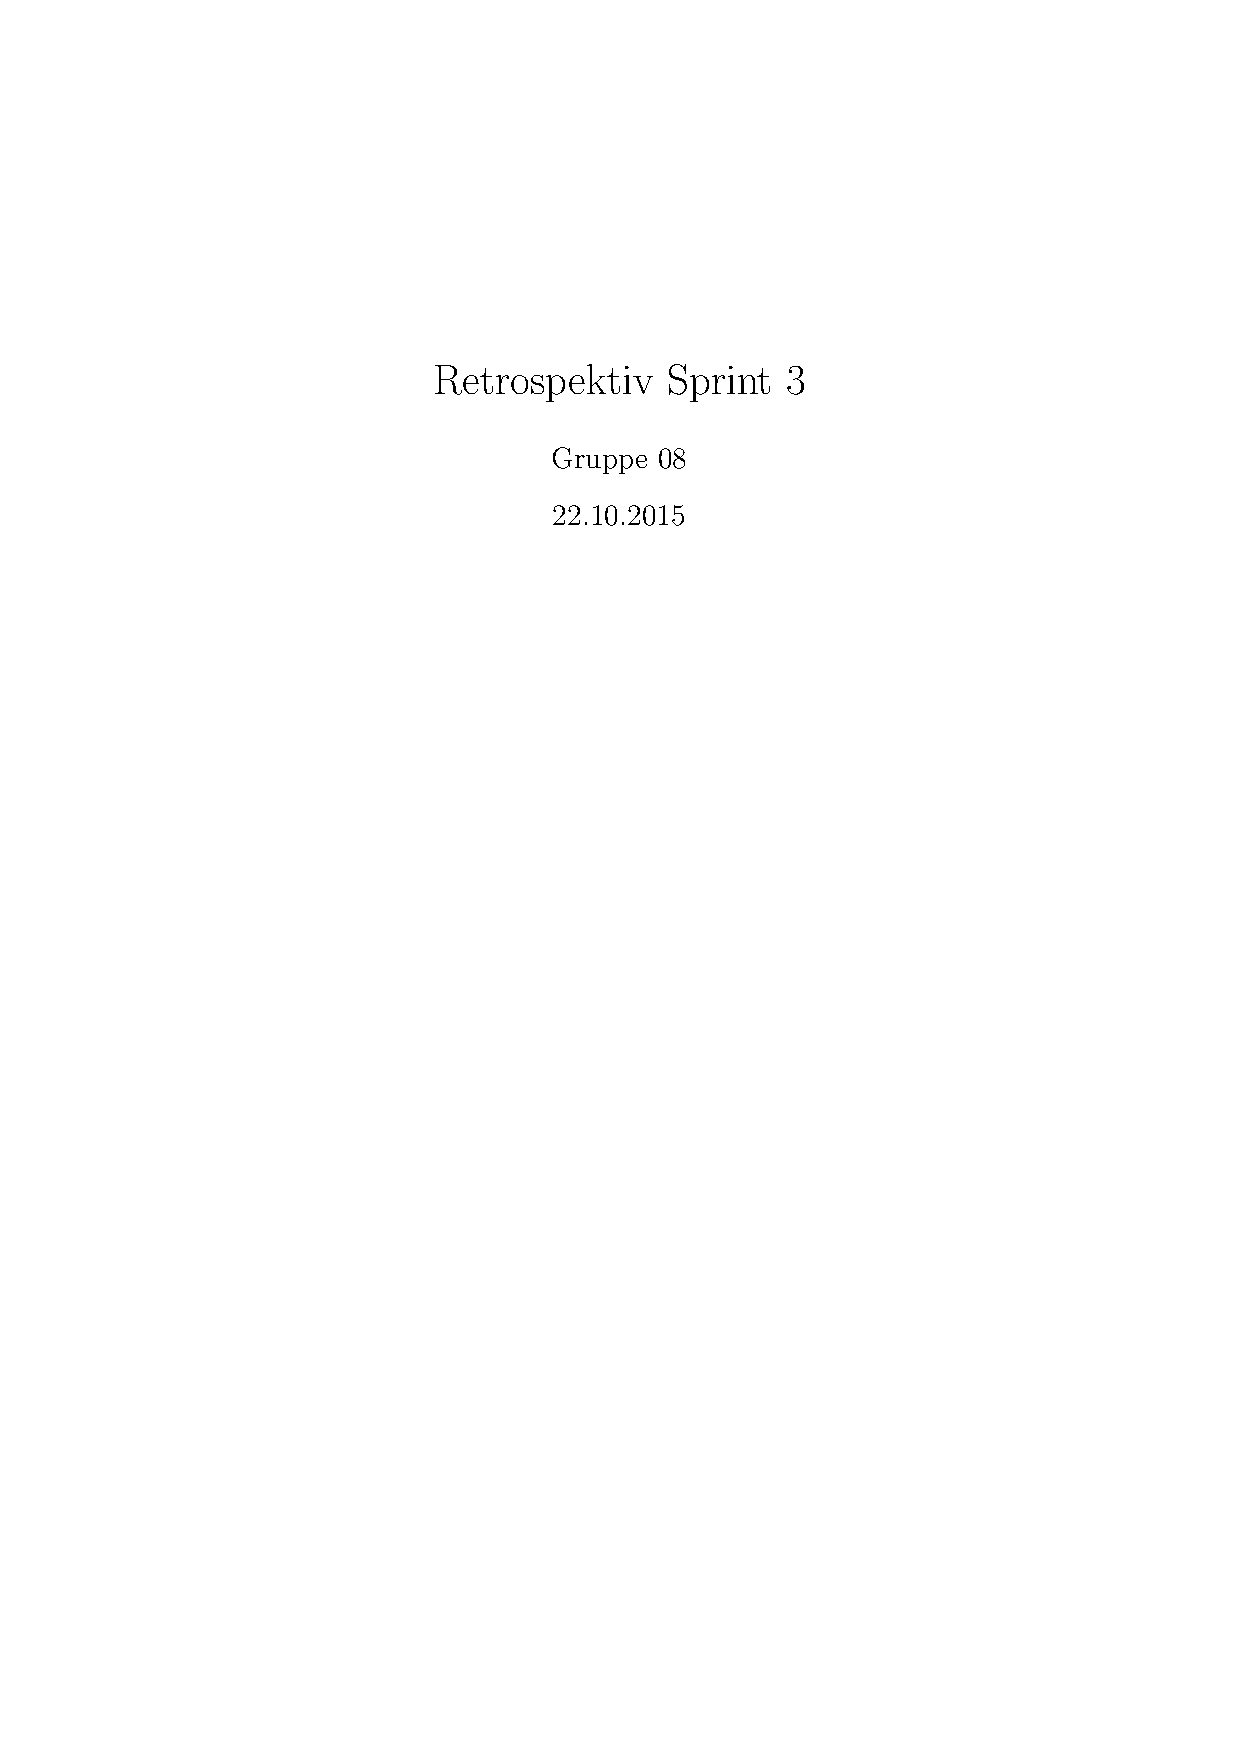
\includepdf[pages={-}]{vedlegg/Retrospektiv/sprint3}

%\addcontentsline{toc}{subsubsection}{Sprint 4}
%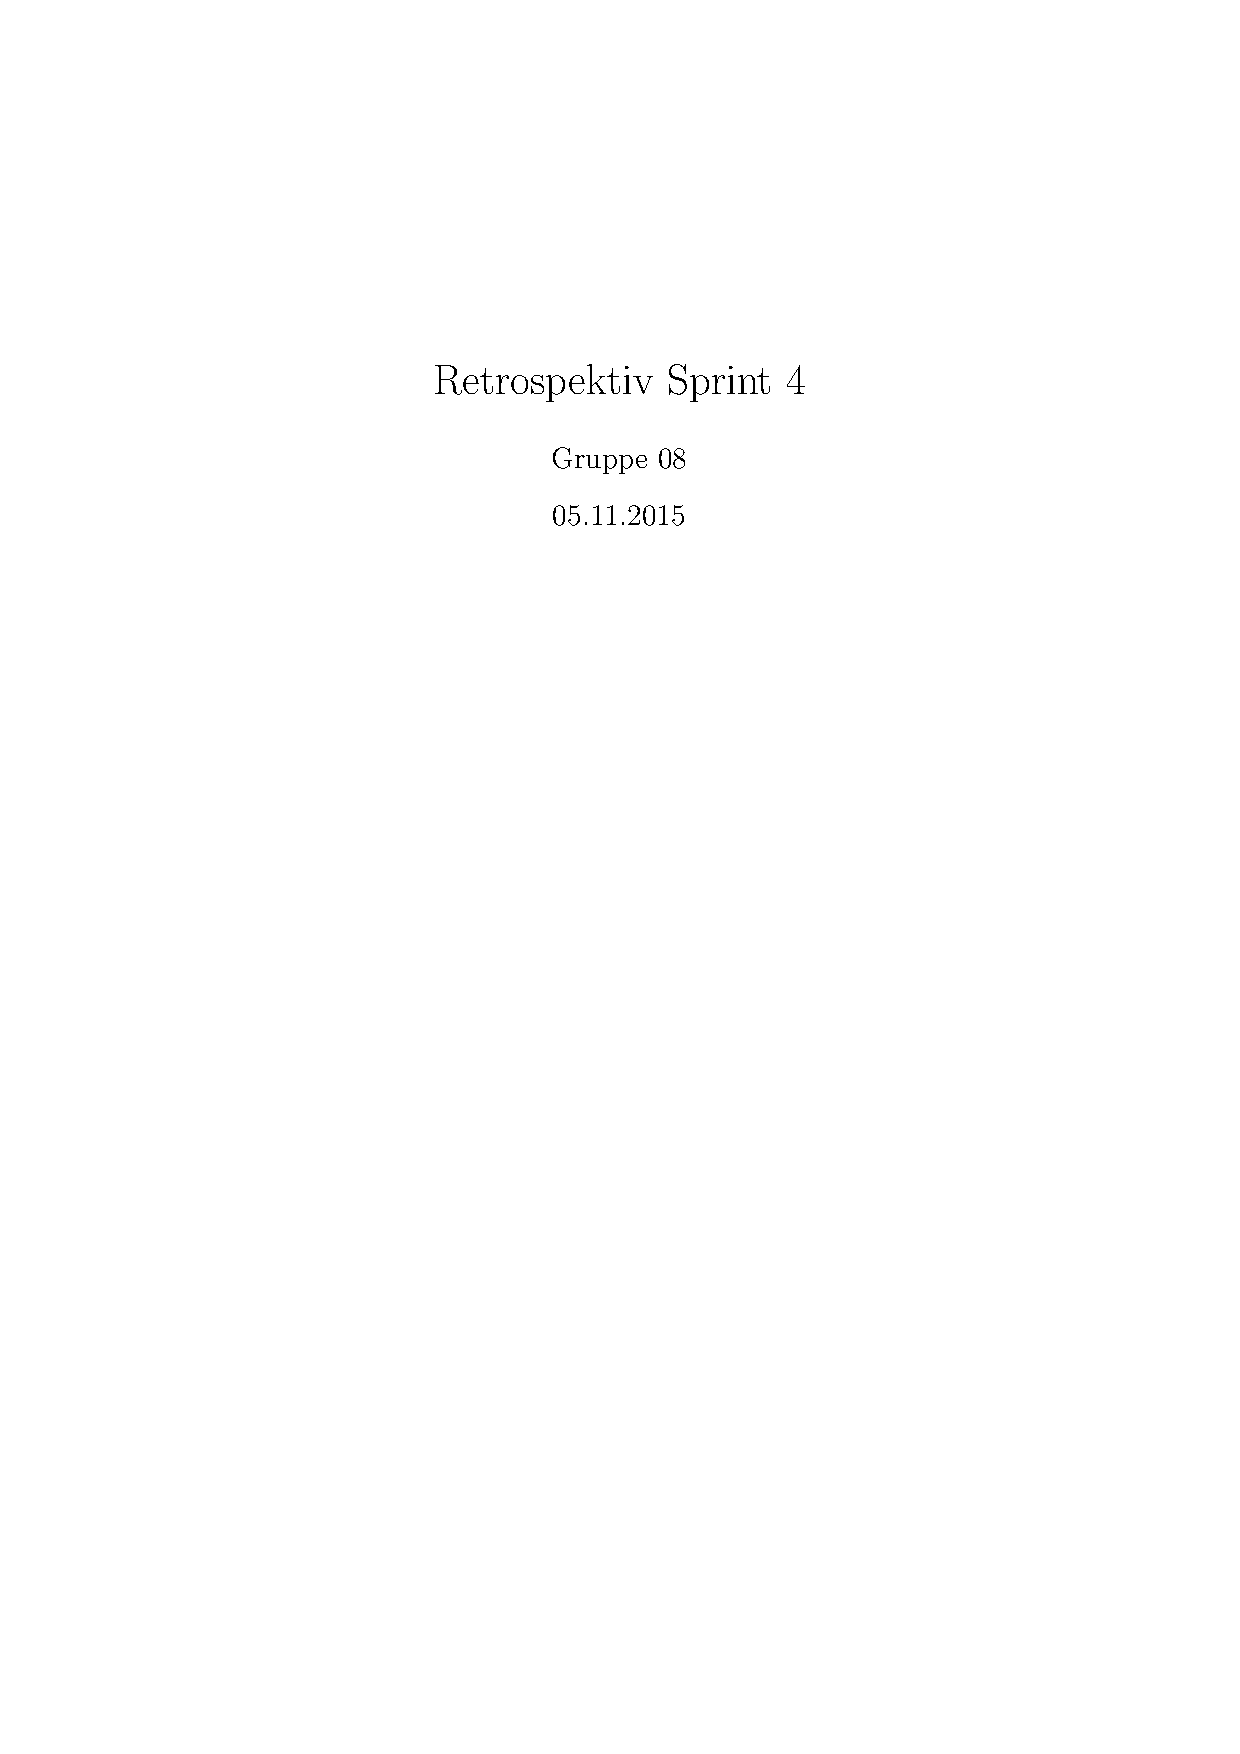
\includepdf[pages={-}]{vedlegg/Retrospektiv/sprint4}

%%RELEASEPLAN
%\addcontentsline{toc}{subsection}{Releaseplan}

%\addcontentsline{toc}{subsubsection}{Releaseplan-v1}
%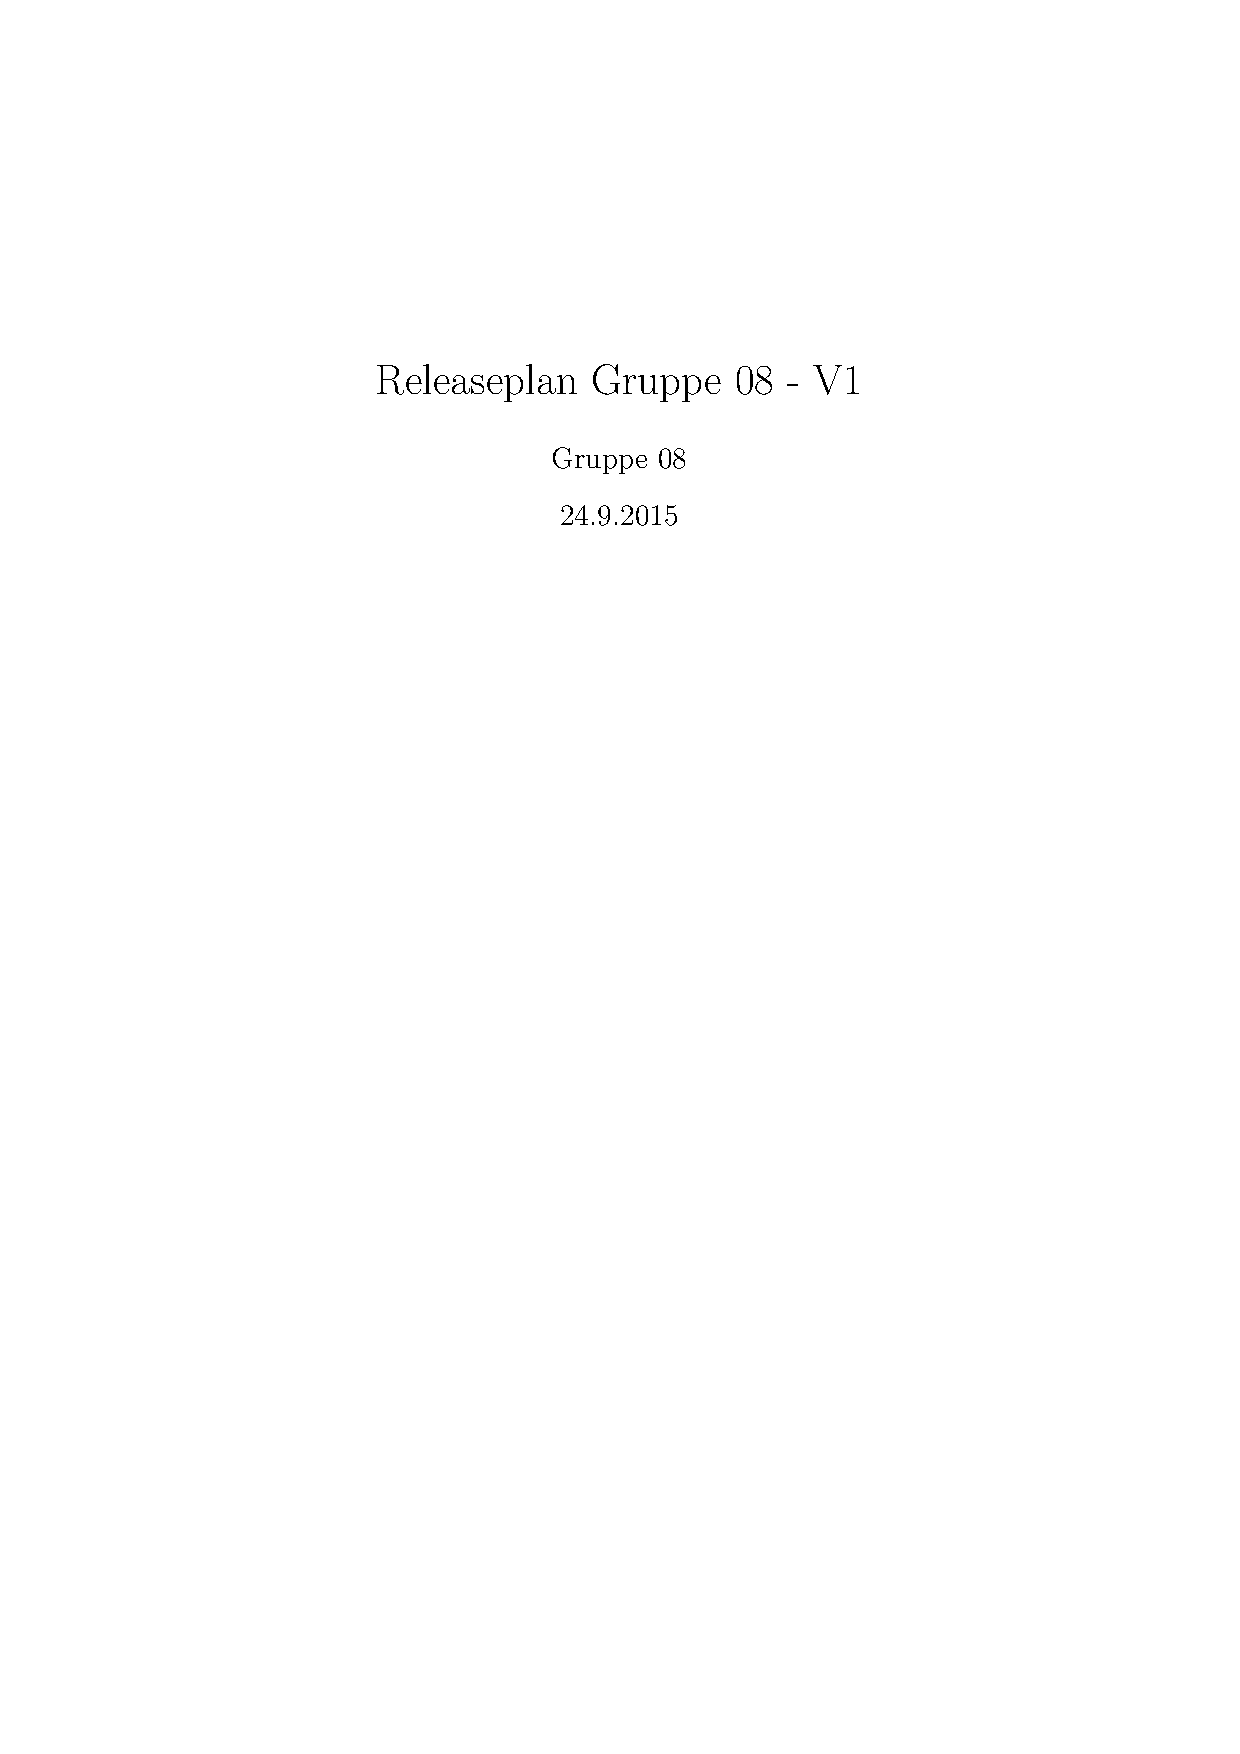
\includepdf[pages={-}]{vedlegg/releaseplan/releaseP1}

%\addcontentsline{toc}{subsubsection}{Releaseplan-v2}
%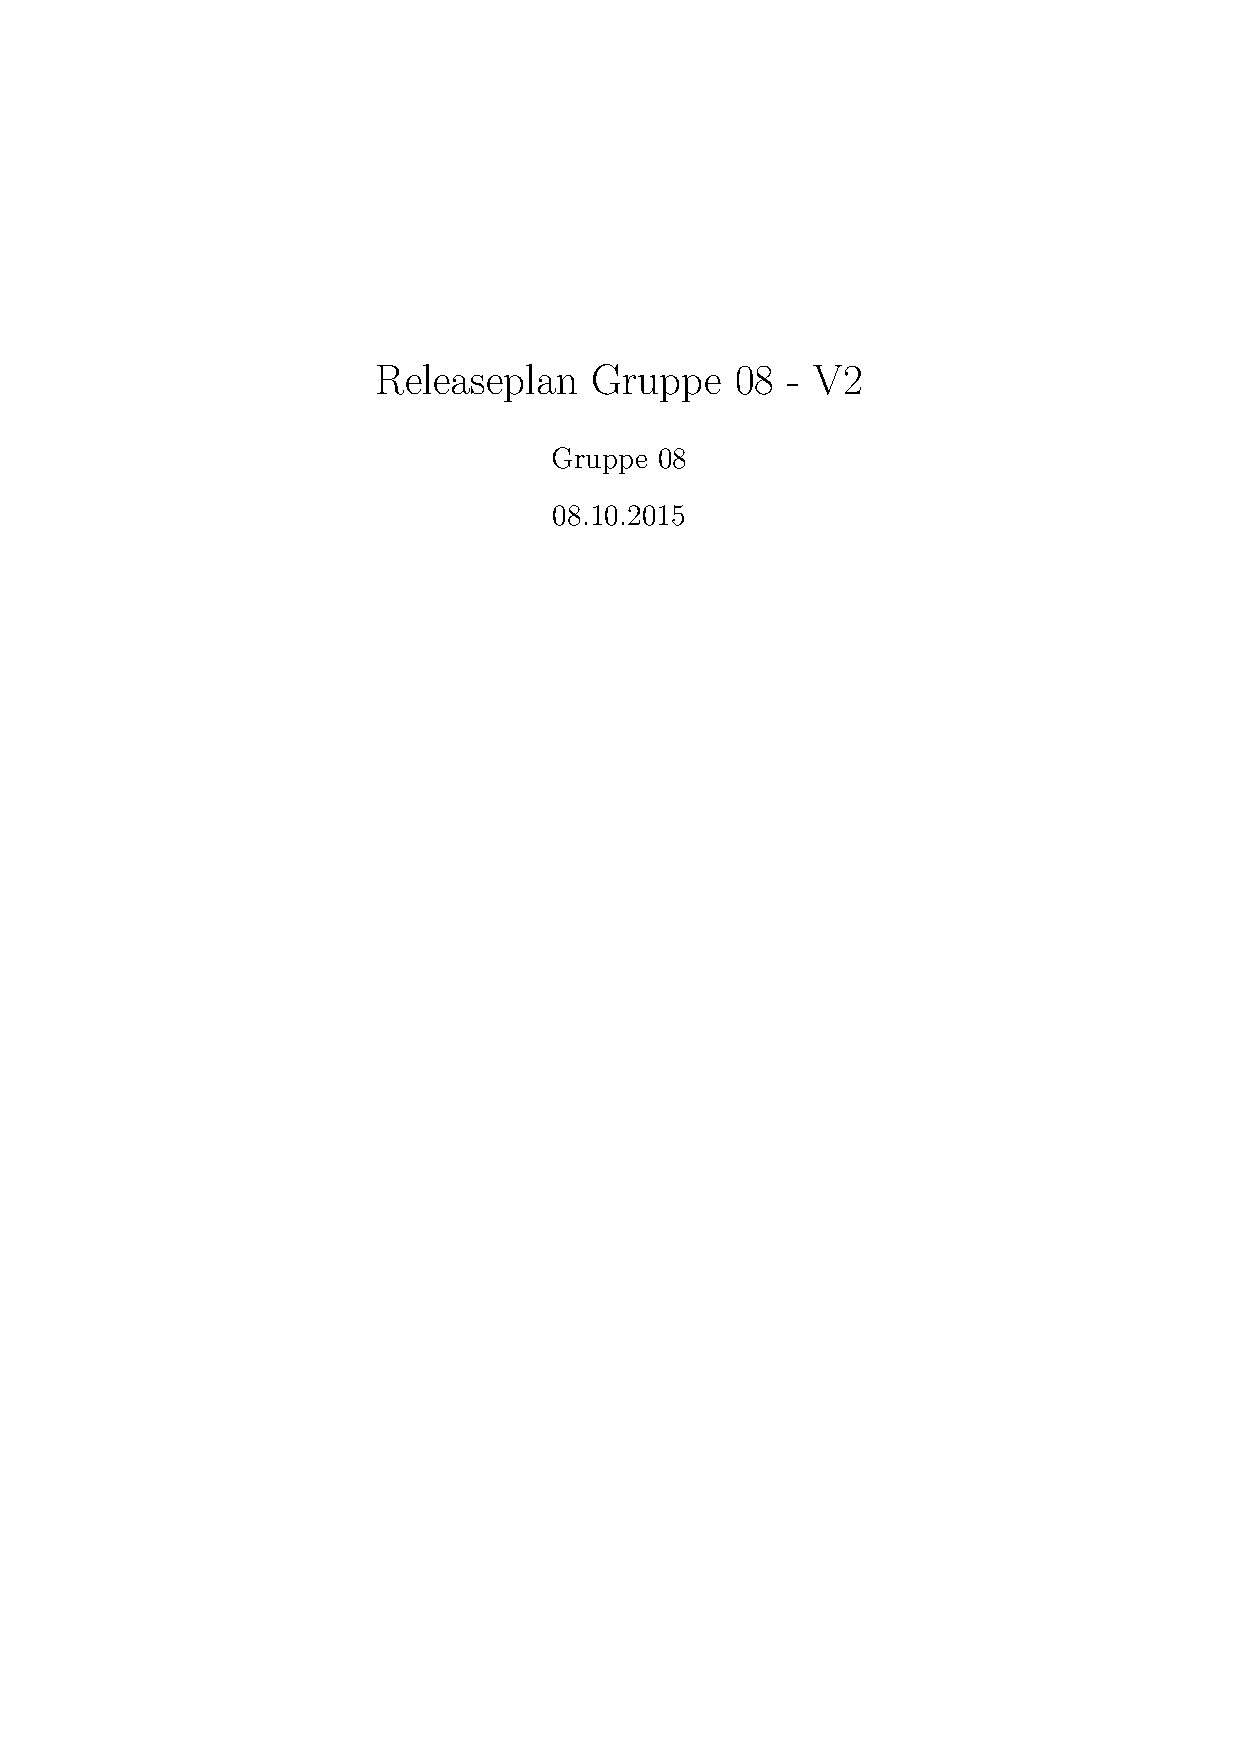
\includepdf[pages={-}]{vedlegg/releaseplan/releaseP2}

%\addcontentsline{toc}{subsubsection}{Releaseplan-v3}
%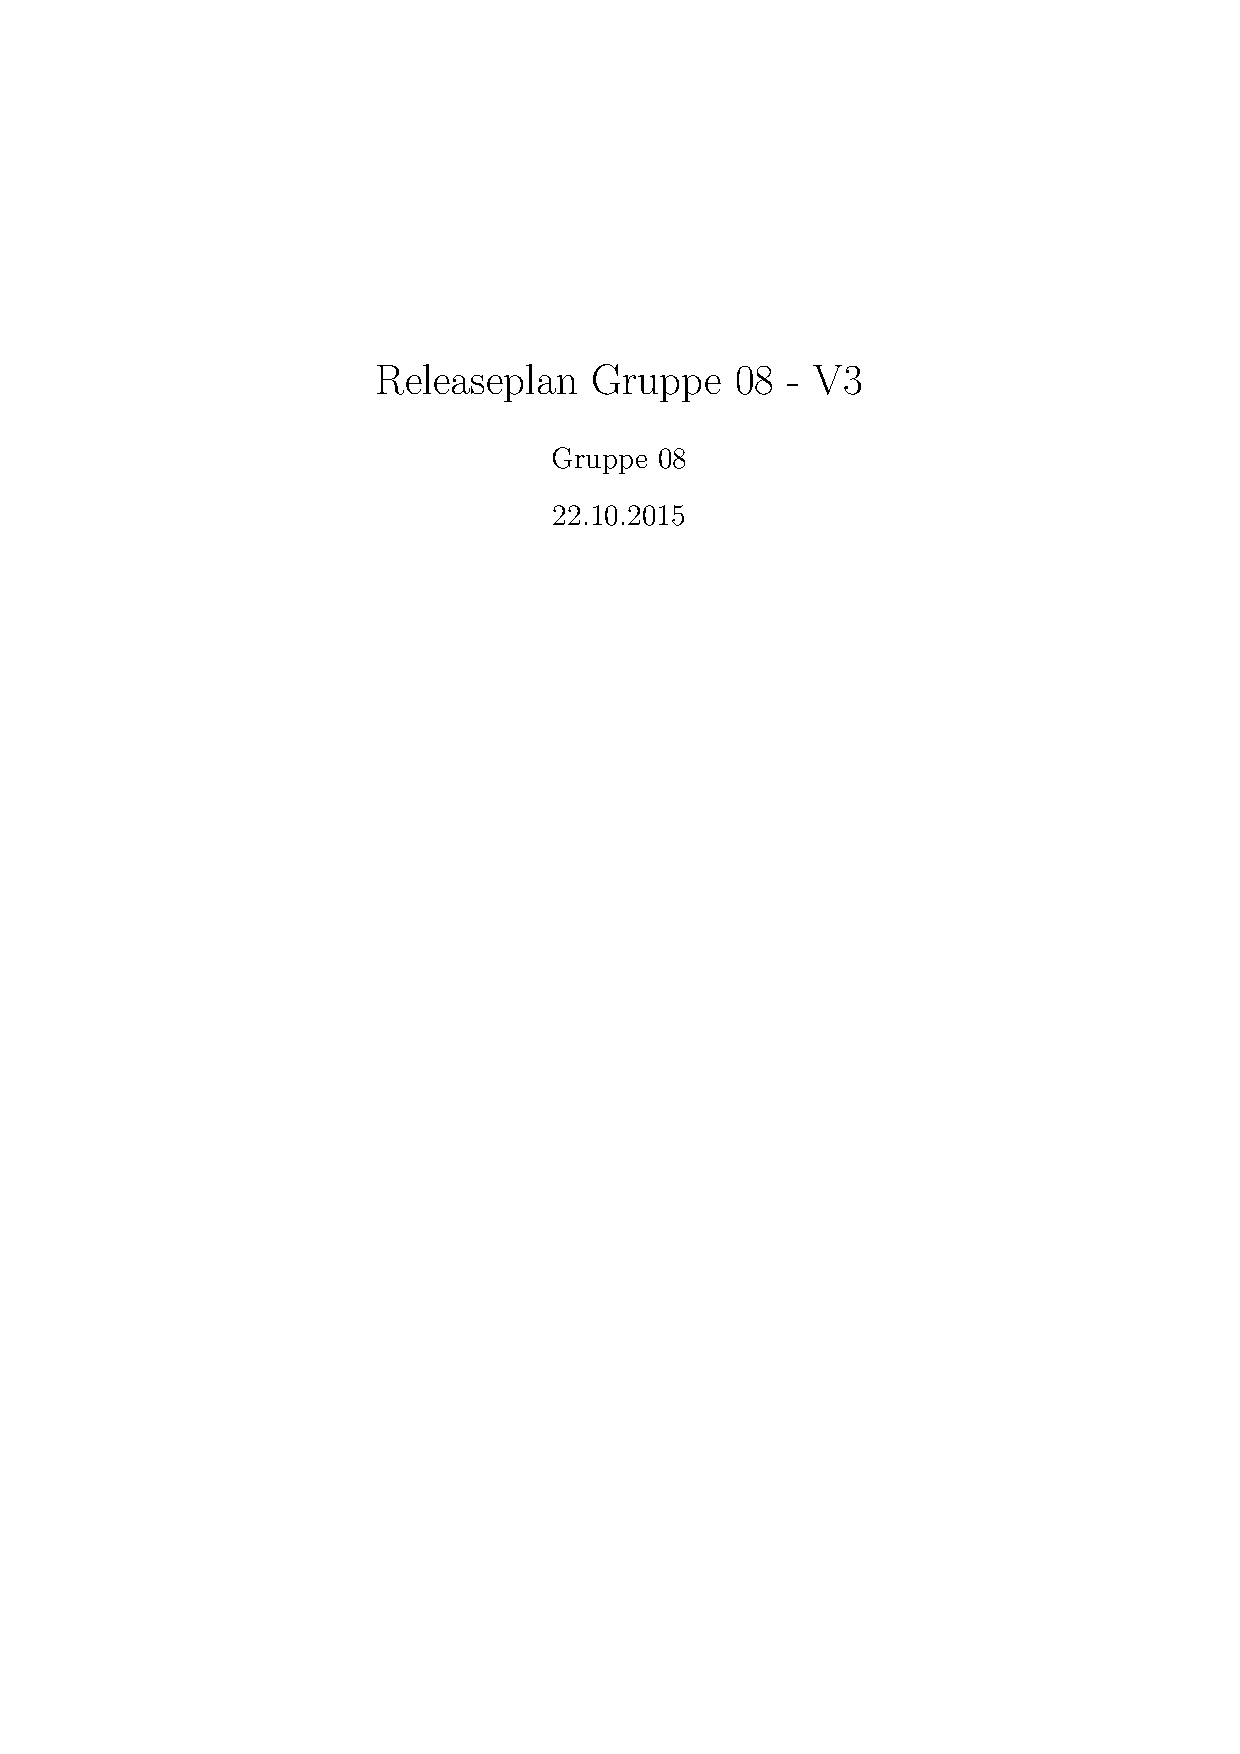
\includepdf[pages={-}]{vedlegg/releaseplan/releaseP3}


\end{document}
